%% Käytä toinen näistä:
%% ensimmäinen, jos käytät pdflatexia, joka kääntää tekstin suoraan 
%% pdf-tiedostoksi (kuvat on oltava jpg- tai pdf-tiedostoina)
%% toinen, jos haluat tuottaa ps-tiedostoa (käytä eps-formaattia kuville,
%% alä käytä ps-muotoisia kuvia!)


%% Käytä näitä, jos kirjoitat englanniksi. Katso englanninokset tiedostosta
%% thesistemplate.tex.
\documentclass[english,12pt,a4paper,pdftex,elec,utf8]{aaltothesis}
%\documentclass[english,12pt,a4paper,dvips]{aaltothesis}
\usepackage{babel}
\usepackage[utf8]{inputenc}
\usepackage{graphicx}
\usepackage[binary-units=true]{siunitx}
\usepackage{textcomp}
%\sisetup{detect-family}
%\AtBeginDocument{\sisetup{math-rm=\mathrm, text-rm=\rmfamily}}

%% Matematiikan fontteja, symboleja ja muotoiluja lisää, näitä tarvitaan usein 
\usepackage{amsfonts,amssymb,amsbsy}
\usepackage[T1]{fontenc}
\usepackage{listings}
\usepackage[super]{nth}
\usepackage{csquotes}
\usepackage{tikz}
\usetikzlibrary{shapes,arrows}
\usetikzlibrary{dsp, chains}
\usetikzlibrary{arrows, decorations.markings}
\DeclareMathAlphabet{\mathpzc}{OT1}{pzc}{m}{it}
\newcommand{\z}{\mathpzc{z}}
\usepackage{pgfplots}
\usepackage{amsmath,bm,times}
\newcommand{\mx}[1]{\mathbf{\bm{#1}}} % Matrix command
\newcommand{\vc}[1]{\mathbf{\bm{#1}}} % Vector command

\usepackage{color} %red, green, blue, yellow, cyan, magenta, black, white
\definecolor{mygreen}{RGB}{28,172,0} % color values Red, Green, Blue
\definecolor{mylilas}{RGB}{170,55,241}

\renewcommand{\labelenumii}{\theenumii}
\renewcommand{\theenumii}{\theenumi.\arabic{enumii}.}

% load package with some of the available options - you may not need this!
\usepackage[framed,numbered,autolinebreaks,useliterate]{mcode}


%% Jos et jostain syystä pidä, miten alla oleva hyperref-paketti käyttää
%% fontteja, värejä yms., käytä tämän paketin makroja muuttamaan
%% fonttimäärittelyt. Katso paketin dokumentaatiota. Paketti määrittelee
%% \url-makron, joten ota paketti käyttöön, jos et käytä hyperref-pakettia.
%%
%\usepackage{url}

%% Saat pdf-tiedoston viittaukset ja linkit kuntoon seuraavalla paketilla.
%% Paketti toimii erityisen hyvin pdflatexin kanssa. 
%%
\usepackage{hyperref}
\hypersetup{pdfpagemode=UseNone, pdfstartview=FitH,
  colorlinks=true,urlcolor=red,linkcolor=blue,citecolor=black,
  pdftitle={Default Title, Modify},pdfauthor={Your Name},
  pdfkeywords={Modify keywords}}

%\usepackage{textcomp}

\usepackage[backend=biber,
style = ieee]{biblatex}
\addbibresource{bibliography.bib}
%% Kaikki mikä paperille tulostuu, on tämän jälkeen
\begin{document}

%% Korjaa vastaamaan korkeakouluasi, jos automaattisesti asetettu nimi on 
%% virheellinen 
%%
%% Change the school field to specify your school if the automatically 
%% set name is wrong
% \university{aalto-yliopisto}
% \school{Sähkötekniikan korkeakoulu}

%% Vain kandityölle: Korjaa seuraavat vastaamaan koulutusohjelmaasi
%%
\degreeprogram{Elektroniikka ja sähkötekniikka}
%%

%% VAIN DI/M.Sc.- JA LISENSIAATINTYÖLLE: valitse laitos, 
%% professuuri ja sen professuurikoodi. 
%%
\department{Department of Automation and Systems Technology}
\professorship{Autonomous Systems}

\univdegree{MSc}
\author{Miika Ihonen}
\thesistitle{Sensor Based Dairy Cow Estrus Detection}
\place{Espoo}

%% Kandidaatintyön päivämäärä on sen esityspäivämäärä! 
%% 
\date{13.11.2017}

%% Kandidaattiseminaarin vastuuopettaja tai diplomityön valvoja.
%% Huomaa tittelissä "\" -merkki pisteen jälkeen, ennen välilyöntiä ja
%% seuraavaa merkkijonoa. 
%% Näin tehdään, koska kyseessä ei ole lauseen loppu, jonka jälkeen tulee 
%% hieman pidempi väli vaan halutaan tavallinen väli.
%%
\supervisor{Prof.\ Arto Visala} %{Prof.\ Pirjo Professori}

%% Kandidaatintyön ohjaaja(t) tai diplomityön ohjaaja(t). Ohjaajia saa
%% olla korkeintaan kaksi.
%% 
%\advisor{Prof.\ Pirjo Professori}
%\advisor{TkT Olli Ohjaaja}
\advisor{M.Sc.\ (tech.) \ Samuli Mäkinen}

%% Aaltologo: syntaksi:
%% \uselogo{aaltoRed|aaltoBlue|aaltoYellow|aaltoGray|aaltoGrayScale}{?|!|''}
%% Logon kieli on sama kuin dokumentin kieli
%%
\uselogo{aaltoRed}{''}

%% Tehdään kansilehti
%%
\makecoverpage



%% Suomenkielinen tiivistelmä
%% Kaikki tiivistelmässä tarvittava tieto (nimesi, työnnimi, jne.) käytetään
%% niin kuin se on yllä määritelty.
%% Tiivistelmän avainsanat
%%
\keywords{Avainsanoiksi valitaan kirjoituksen sisältöä keskeisesti kuvaavia
käsitteitä}
%% Tiivistelmän tekstiosa
\begin{abstractpage}[finnish]
  Tiivistelmässä on... 
\end{abstractpage}

%% Pakotetaan uusi sivu varmuuden vuoksi, jotta 
%% mahdollinen suomenkielinen ja englanninkielinen tiivistelmä
%% eivät tule vahingossakaan samalle sivulle
%%
\newpage
%
%% Opinnäytteen ostikko englanniksi. Poista, jos et tarvitse sitä.
\thesistitle{Thesis template}
%\supervisor{Prof.\ Pirjo Professori}
%\advisor{D.Sc.\ (Tech.) Olli Ohjaaja}
\advisor{M.Sc.\ Samuli Mäkinen}
\degreeprogram{Electronics and electrical engineering}
\department{Department of Radio Science and Technology}
\professorship{Circuit theory}
%% Abstract keywords
\keywords{Resistor, Resistance,\\ Temperature}
%% Abstract text
\begin{abstractpage}[english]
Your abstract in English. Try to keep the abstract short, approximately 
 100 words should be enough. Abstract explains your research topic, 
 the methods you have used, and the results you obtained.  
\end{abstractpage}

%%% Force new page so that the Swedish abstract starts from a new page
%\newpage
%%
%%% Ruotsinkiellinen tiivitelmä. Poista, jos et tarvitse sitä.
%%% 
%%% Opinnäytteen ostikko ruotsiksi.
%\thesistitle{Arbetets titel}
%%\supervisor{Prof.\ Pirjo Professori}
%\advisor{TkD\ Olli Ohjaaja} %
%%\advisor{M.Sc.\ Tina Tutkija}
%\degreeprogram{Elektronik och elektroteknik}
%\department{Institutionen för radiovetenskap och -teknik}%
%\professorship{Kretsteori}  %
%%% Abstract keywords
%\keywords{Nyckelord p\aa{} svenska,\\ Temperatur}
%%% Abstract text
%\begin{abstractpage}[swedish]
% Sammandrag p\aa{} svenska.
% Try to keep the abstract short, approximately 
% 100 words should be enough. Abstract explains your research topic, 
% the methods you have used, and the results you obtained.  
%\end{abstractpage}

%% Note that if you are writting your master's thesis in English, place
%% the English abstract first followed by the possible Finnish abstract


%% Esipuhe 
%%
\mysection{Prologue}

The accomplishment of this master's thesis has been a long journey with various phases. My youngest son was born in the very beginning of this project and changed the ordinary life of our entire family. Furthermore, the project was delayed in result of the slow process of data recording. Finally, after the first birthday of my youngest son my thesis is complete. Therefore, I humbly praise my dear family for the patience and support among this long project.

\vspace{5cm}
Otaniemi, 13.11.2017

\vspace{5mm}
{\hfill Miika S.\ Ihonen \hspace{1cm}}



%% Pakotetaan varmuuden vuoksi esipuheen jälkeinen osa
%% alkamaan uudelta sivulta
\newpage


%% Sisällysluettelo
\thesistableofcontents


%% Symbolit ja lyhenteet
\mysection{Symbols and Abbreviations}


\subsection*{Symbols}

\begin{tabular}{ll}
$g$          & acceleration unit $ \approx 9.81 \mathrm{[m/s^2]}$\\
\end{tabular}

\subsection*{Operators}

\begin{tabular}{ll}
$\sum_i $                       & sum over the index $i$ \\
\end{tabular}

\subsection*{Abbreviations}

\begin{tabular}{ll}
MCU & Micro-Controller Unit (or micro-controller) \\
SD & Secure Digital \\
SDHC & High Capacity Secure Digital \\
SDXC & Extended Capacity Secure Digital \\
SPI & Serial Peripheral Interface bus \\
I$^2$C & Inter-Integrated Circuit bus (also IIC) \\
EEPROM & Erasable Programmable Read-Only Memory \\
SRAM & Static Random-Access Memory \\
FIR & Finite Impulse Response \\
IIR & Infinite Impulse Response \\
FIFO & First In, First Out \\
IDE & Integrated Development Environment \\
FFT & Fast Fourier Transform \\
RISC & Reduced Instruction Set Computer \\
CISC & Complex Instruction Set Computer \\
USB & Universal Serial Bus \\
ISR & Interrupt Service Routine \\
I/O & Input/output \\
LSB & Least Significant Bit \\
MSB & Most Significant Bit \\
\end{tabular}



%% Sivulaskurin viilausta opinnäytteen vaatimusten mukaan:
%% Aloitetaan sivunumerointi arabialaisilla numeroilla (ja jätetään
%% leipätekstin ensimmäinen sivu tyhjäksi, 
%% ks. alla \thispagestyle{empty}).
%% Pakotetaan lisäksi ensimmäinen varsinainen tekstisivu alkamaan 
%% uudelta sivulta clearpage-komennolla. 
%% clearpage on melkein samanlainen kuin newpage, mutta 
%% flushaa myös LaTeX:n floatit 
%% 
\cleardoublepage
\storeinipagenumber
\pagenumbering{arabic}
\setcounter{page}{1}


%% Leipäteksti alkaa
%%

\clearpage
%-----------------------------------------------------------------------%
\section{Introduction}
\thispagestyle{empty}

People have been using milk as a source of nutrition since the early state of animal husbandry. The researches have shown that the drinking of milk started 8000 years ago in the present Turkey area. Ever since the dairy farming has spread all over the world. Meanwhile, the spectrum of the available dairy products and fabrication techniques have been increasing. In the staring time of cattle keeping, the headcount was small, and it served only a family or a local community. However, since industrialization the farm sizes have increased whereas, the number of farms begun to decrease. Same trend has been going on thereafter. Nowadays, strict competition in local and global markets has driven the dairy farmers in financial challenges. Consequently, human labor has become an expensive recourse cutting the profitability. Moreover, it has caused the increase of the workload of the farmers. Thus, they have less time to spend with the cattle observing the status of estrus and health issues. Punctual estrus detection is fundamental factor in keeping the calving interval within the optimal range. Extended calving intervals have direct affect in milk yield and the profitability of the farm. In Finland, the average calving interval has already exceeded 400 days whereas, 360 days is the optimal and recommended interval. Traditionally, estrus and health issues have been detected sight-wise by the cattle tender. This method is time consuming and nowadays considered inefficient. However, such symptoms as lameness are still difficult to detect with sensor-based solutions. By contrast, lameness is visually rather easy to detect. Nevertheless, one of the objective of sensor-based technologies is to detect health issues before they escalate into sever conditions such as lameness.

Currently, there are numerous technological solutions available as an alternative to human labor. However, they are relatively expensive investments and their actual payback time is difficult to define. Therefore, specially many small farms have postponed the investments to acquire the modern technological aids in cattle monitoring. Additionally, even large farms in developing countries are in the same state and they still rely on human labor and traditional methods. In addition to the high cost and long payback time, the functionalities and the performance level of the solutions can vary significantly. Thus, achieving of complementary solution for dairy cow monitoring is rather challenging. Typically, these commercial solutions offer aids for estrus detection and general health tracking. Furthermore, the current solutions tend only to trigger alarms instead of providing accurate health status. Thus, cattle tender is still required to make health estimation and decide whether a veterinarian is required for help or not.

Based on this background information, the rigorous detection of estrus for insemination is one of the most critical issues in nowadays dairy farming. Thus, this study aims to develop and evaluate an effective algorithm for dairy cow estrus detection. In addition to effective algorithm, it shall be suitable for low-cost consumer level hardware components. Conventionally, the cattle tender monitors the cattle and detects the estrus behavior. That is, a cow being mounted by other cows is considered as secure sign of ongoing estrus. There are additional behaviors giving a hint of ongoing estrus. However, confident detection requires several occasions of these other behaviors. Sensor-wise detection of being mounted by others seem quite challenging objective. Thus, another approach shall be considered in this study. Luckily, a highly active period of proestrus leads the estrus. Sensor-wise, activity on motion is more detectable feature. Therefore, the use of accelerometer as the fundamental sensor in these applications is highly reasonable. Additionally, detection of proestrus provides the farmer more time to be prepared for the insemination before the actual estrus. Unfortunately, this approach does not apply on cows in tie-stall because they are not able to behave according their species. Thus, only loose-housed cows are considered in this study. However, the results of this study could be adoptable for beef cattle as well as other animal species. Nevertheless, these options are not in the scope of this study. In addition to the active behavior of the cow, its body temperature rises during the estrus. Therefore, some commercial solutions include body temperature measurement. Similarly, the hardware solution in this study includes a temperature sensor and the purpose of it is to confirm or reject the detected estruses. Nevertheless, the accelerometer is considered as the only fundamental component in estrus detection in this study.

In this study, the focus of the algorithm evaluation in is in reliability and punctuality. Therefore, the algorithm shall not trigger false estrus or miss a true estrus either. Additionally, the timing shall remain within reasonable tolerance.  Thus, the resulting algorithms shall be able to detect estrus in real-time. In addition to these requirements, the algorithm shall be stand-alone solutions and suitable for low-cost consumer level micro-controller based devices. Therefore, in this study we use common low-cost components in the sensor device hardware design. However, in this kind of wearable battery-based solutions the high capacity batteries expensive and their cost may exceed the price of the other hardware components. Thus, low energy consumption is frequently considered in the discussions of this study. In addition to the estrus detection, the secondary objective of this study is in behavior monitoring. There are various observable behaviors such as walking, eating and ruminating. However, the behavior monitoring is only the secondary objective in this study. Thus, we will study the topic only briefly and discuss of the future options as conclusions.

Efficient real-time data analysis, algorithm development and testing are an absurd approach to the scope of this study. Specially, when the estrus cycle of a cow lasts approximately 21 days and the phases of proestrus and estrus several hours. Therefore, it is essential to use recorded sensor data instead in algorithm development and testing. Consequently, implementation of suitable data recording software is one of the core topics in this study. Furthermore, properly implemented data recording application gains benefits for possible following studies as well. The data recording application shall be implemented on similar cost-efficient hardware platform as the actual estrus detection algorithm. However, in contrast to software development, the designing of the hardware is not in the scope of this study. However, introduction of the hardware platform used in this study is mandatory preliminary knowledge ad it is required in the software implementation. Therefore, we will discuss of the main hardware components and their functionalities in reasonable detail. Despite the requirements of real-time punctuality, the real-time testing of the estrus detection algorithms is excluded from this study. By contrast, the algorithms shall be implemented and tested with an appropriate computer software  and the results are discussed with care in the results section. Nevertheless, the convertibility of the algorithms are considered throughout the development process. However, the implementation of the actual algorithms on the micro-controller is not discussed in this study.


%Despite the real-time punctuality of the resulting algorithms, testing of the algorithms on-site is not in scope of this study. Conversely, the algorithms shall be developed and tested with a suitable computer software. The algorithm development requires real cow data from a dairy farm. Therefore, implementation of a suitable data recording software for a low-cost micro-controller device is one of the core topics in this study. 
%
%
%Kerro menetelmistä.
%
%Onko muita rajauksia?
%
%Puuttuuko jotain muita perusteluja tutkimuksen tekemiselle, valinnoille yms?



\clearpage 

 %-----------------------------------------------------------------------%
\section{Background} \label{backgroundsection}
 
Originally, humans were hunter-gatherers who obtained food by collecting plants and pursuing wild animals. The methods for acquiring food have changed substantially since the beginning of the agriculture. That is, plants and animals are grown centralized in large farms instead of numerous small producers. The animal husbandry has been estimated to been started more than 10,000 years ago in western Asia. Accordingly, goats were among the first domesticated animals in human history \cite{ancienthistoryofmilk}. Thereafter, people have been domesticating other species e.g. cows, sheep and pigs for milk, meat and other animal products. In addition to the quantity of various species, the headcount has been increasing with the population. Furthermore, the industrial revolution has started a trend of growing farm sizes and a loss of smaller farms. Recently, the total headcount of the world has been estimated almost up to 1,000 million heads in 2016 \cite{livestockandpoultry}.

Nowadays, the cattle breeding is divided into two trends of beef and dairy farming. As a result, the breeds of beef cattle and dairy cattle are considerably different in physics and by nature. The beef breeds are more muscular whereas milk breeds are tamer. Moreover, the scope of beef breeding is in rapid brawn growth, while high milk yield is the target of the dairy cattle breeding. Despite the same origin of the breeds, they are as distinct as different species. Therefore, the scope of this study is only in dairy farming. Accordingly, the following subsections will discuss briefly of the history and the basics of the modern dairy farming \ref{dairyfarmingsection}. Furthermore, we will survey through the life of a cow \ref{dairycowsection} and discuss of related issues. Additionally, we will focus in two fundamental cycles in the life of a dairy cow, estrus cycle and lactation cycle \ref{lactationandestruscyclessection}. These cycles are directly related to the milk yield and profitability of the dairy farm. In addition to the discussions of the dairy cow, we will take an overview on dairy cow monitoring \ref{currentsolutionssection}. The overview includes as well as traditional methods as currently available technological aids. Lastly in the background section, we will survey through the most recent research and studies in dairy cow monitoring \ref{researchandstudiessection}. In the survey, we will focus specially in wearable sensor devices and behavior monitoring.

%-----------------------------------------------------------------------%
\subsection{Dairy Farming} \label{dairyfarmingsection}

As discussed in previously, the origins of animal husbandry are over 10,000 years old. Whereas, the drinking of milk started 8,000 years ago in present Turkey area. Thousand years later, dairy farming started to spread into Europe and thousand years after that into Africa \cite{ancienthistoryofmilk}. Thereafter, dairy farming has spread all over the world. Meanwhile, the variety of dairy products has exploded simultaneously. In result, there are numerous different milk, cheese and yogurt products as well as other dairy refinements. Additionally, dairy products have an essential part in human nutrition nowadays. Furthermore, milk and other dairy products are produced more than ever before. Concurrently, the farm headcounts have been increasing whereas the number of farms has started to decrease. Alone in Finland, there were total of 909,000 cows of which 282,000 milking cows. Meanwhile, 7890 farms delivered milk to milk processing plants in the end of the year 2015. As a result, the average yield of a farm was 279 thousand liters whereas the average yield of a cow was 8300 liters. Accordingly, the total milk yield in Finland was 2365 million liters in 2015 \cite{ruokajaluonnonvaratilastot2016}. Correspondingly in the Unites States of America, there were more than 89 million cows and calves of which more than 9 million were milking cows in 2014. The corresponding cash income of the dairy farms was more than 49,349 million dollars in 2014 in the USA \cite{agriculturalstatistics2015}.


Originally, cows were wild pasture animals and, afterwards,  domesticated by humans. At the beginning of animal husbandry, the people was migrating nomads. Therefore, the cattle traveled with people. Eventually, people started farming and settled in constant regions with their animals. First, the animals were held in yards but then people started to build structures for protection and easier keep of the animals. Next, people started to keep their cattle inside buildings. In linear pottery culture, people and animals lived together inside longhouses. Finally, people started to build separate buildings for their animals. Special building for keeping cows are called cowsheds. Currently, the cowsheds are divided in two types of tie-stall and loose-housed cowsheds \cite{lehmahavaintoja}. In general, tie-stall cowsheds are smaller and, therefore,  tighter than loose-housed cowsheds. Furthermore, cows are not allowed to move freely in tie-stall. Conversely, In loose-housed cowshed cows are allowed to move freely round the clock. Additionally, they may have free access to pasture in some solutions. Recently, the tie-stall cowsheds have been under critique. That is, the cows are not able to behave as social animals. Additionally, the monitoring and health keeping of the cows is more difficult in tie-stalls. Therefore, most of the new-builds are rather loose-housed than tie-stall cowsheds. In addition, it is considered the cows of being happier and healthier in loose-housed cowsheds. 

\begin{figure}
%[thb]
\centering
\includegraphics[width = 0.75\textwidth]{figures/tie-stall-barn.jpg}
\caption{Cows in a tie-stall-cowshed \cite{tiestallbarnpicture}. Cows are tied in stall and they are not able to move freely. They also have less space than in a loose-housed cowshed.}
\end{figure}

\begin{figure}
%[thb]
\centering
\includegraphics[width = 0.75\textwidth]{figures/free-stall-barn.jpg}
\caption{Cows in a loose-housed-cowshed \cite{freestallbarnpicture}. Cows are able to move freely and act as social animals.}
\end{figure}


%-----------------------------------------------------------------------%
\subsubsection{Dairy Cow} \label{dairycowsection}


Previously, we surveyed through the history of animal husbandry and discussed of the beginning milk producing. Additionally, we introduced such modern cowsheds as tie-stall and loose-housed cowsheds. Correspondingly, this subsection will focus on the dairy cow itself in general level whereas, the following subsection will focus on such milk yield related cycles as estrus and lactation cycles. 

Inherently, cows are plain and herd animals. Moreover, they live in hierarchy \cite{julkaisuja52}. In large herds they form smaller groups where they do their daily activities such as eat and rest together \cite{julkaisuja52} \cite{lehmahavaintoja}. Typically, cows lay down approximately from \SI{11}{\hour} to \SI{12}{\hour} every day. They doze standing and sleep lying \cite{julkaisuja52}. Meanwhile, they stand up and change their pose or place several times \cite{luomunaudanruokinta}. Additionally, they walk between haunts and watering places. Thus, in loose-housed cowshed a cow may walk from  \SI{400}{\metre} to \SI{800}{\metre} every day \cite{luomuopas}. By contrast, on pasture their daily walking range may exceed several kilometers \cite{luomuopas} \cite{julkaisuja52}. However, cows are very cautious animals. Thus, they avoid insecure circumstances such as slippery ground or high steps, hence they get easily injured in such places. In result, insecure circumstances can reduce their daily walks significantly. Nevertheless, Walking enforces their health, increases their hormonal activity and metabolism \cite{luomuopas}. Conversely, all the injuries effects to their health and consequently to the milk yield and profitability  of the farm \cite{lehmahavaintoja}. Additionally,  free access to fresh and clean water is vital for the cows. \cite{luomuopas} 

In contrast to their normal actions and daily routines, exceptional behavior can indicate a situation which requires the cattle tender to act. Various health issues appear in exceptional behavior and they are the most alarming  situations in dairy farming. Injuries and sicknesses can easily escalate into sever conditions of which the cow may not recover. Anyhow, severe sickens and in advance slaughtered animal cause significant financial losses and are always avoidable situations. In addition to health issues, some of the exceptional behaviors are part of their life cycles. That is, the estrus behavior. In contrast to the sicknesses, the cow in proestrus becomes highly active. Also, the signs of estrus are important indicators to the cattle tender. Nevertheless, we discuss the phases of estrus more in detail in the following subsection.


% Tänne vähän lisää tietoa lehmien terveysongelmista, kuten ontumisesta, sorkkahommista ja ruoansulatusvaivoista. 
 
% Tähän alkuun vielä jotakin lehmän perustietoja, kuten arvio rotujen määristä. Lehmän keskimääräinen paino, koskeus, pituus jne. Ehkä myös maininta siitä, kuinka paljon lehmä tarvitsee tilaa mm. laskeutumiseen ja ylösnousuun. 



%-----------------------------------------------------------------------%
\subsubsection{Lactation and Estrus Cycles} \label{lactationandestruscyclessection}

In previous subsections, we discussed of dairy farming and dairy cow in general. Consequently, in this section we will proceed the discussion into lactation and estrus cycles. The lactation cycle is emphatically related to the milk yield and thus, to the profitability of the farm. Basically, the lactation cycle means the period between two calves. Thus, it is also called as calving period. After calving a cow begins to lactate, which is the primary purpose of a dairy cow \cite{lehmahavaintoja}. Therefore, the calves are a secondary product in dairy farming. Furthermore, the destiny of calves is not in scope of this study. Nevertheless, the milk yield of a cow increases during the first weeks after the calving. However, after few weeks the milk yield begins to decrease as it is illustrated in figure \ref{lactationapproximation}. The lactation curve is a coarse estimation of typical milk yield versus the weeks from calving and it should not be considered as an exact knowledge. Nevertheless, it is not cost-efficient to keep on milking the cow infinitely, hence the milk yield decreases at too low level. Therefore, a cyclic calving is preferred solution in order to maintain proper milk yield and descent profitability. However, the cow will stop milking before calving. This is called a dry period. The dry period provides the cow and her udder time to prepare for the next lactation. However, the dry  period and decreased lactation forms a dilemma where too short as well as too long lactation cycle reduces the total milk yield. In general, the recommended calving interval is roughly in 360 days. Additionally, some researches have shown that the milk yield of a cow increases after each calving. Thus, it supports the concept of regular calving \cite{lehmientuotoskasvaa}.

 \begin{figure}
 %[thb]
 \centering
 \begin{tikzpicture}
    \begin{axis}[
        xlabel=weeks from calving,
        ylabel=milk yield (kg)]
    \addplot[smooth, blue] plot coordinates {
    	(0,15)
        (1, 30)
        (2, 38)
        (4, 40)
        (6,	39)
        (8,	38)
        (10, 37)
        (12, 35)
        (16, 33)
        (20, 30)
        (24, 27)
        (28, 25)
        (32, 22)
        (36, 21)
        (40, 20)
    };
    \end{axis}
    \end{tikzpicture}
    \caption{An illustrative lactation curve of a dairy cow representing the relation between the weeks in milk and the milk yield. After the beginning of the lactation, the milk yield reduces in the function of time \cite{lactationcurve}.} \label{lactationapproximation}
 \end{figure}

However, in the recent years, the calving interval has been increasing globally. Alone in Finland, the average calving interval has extended up to 400 days and it has affected to the milk yield and profitability. The consequences are already remarkable. Therefore, there has been discussions of the root causes for the extended calving interval. In general, the farm sizes have been increasing and the cattle tenders have more work to do and less time for observing the cows. Thus, it has been more difficult for them to detect estrus behavior sight-wise. In result, there are missed estruses and insemination. Consequently, this trend has forced the farmers to seek technological aids for a punctual estrus detection. Therefore, the primary objective of this study is in developing of effective estrus detection algorithms for wearable low-cost sensor device.

In addition to the lactation cycle, it is necessary to discuss of the estrus cycle as well. The estrus cycle is the period between ovulations. Precisely, the estrus cycle is considered to begin from an ovulation and end to the beginning of the next. The normal duration of a cow estrus cycle is approximately 21$\pm$3 days. Typically, the estrus lasts from 12 to 16 hours \cite{julkaisuja52}. Moreover, a bull may detect an estrus already 2 days in advance. Furthermore, the estrus is the time frame when the cow is ready to mate or being inseminated. In spoken language, the estrus is also called as standing heat, hence, the cow stands still and allows being mounted by other cows. Traditionally, a cow being mounted by others has been considered as certain sign of ongoing estrus. However, the occasions of being mounted are rare and consequently, the cattle tender does not notice the present estrus at all. However, a proestrus period lead the actual estrus. A cow in proestrus behaves restlessly and usually it attempts to mount other cows. However, the other cows do not allow being mounted unless they are in estrus themselves. Typically, the duration of proestrus is from 9 to 18 hours \cite{lehmahavaintoja}. In contrast to the actual estrus, the highly active period of proestrus provides a sufficient detectable behavior sensor-wise. Thus, that is the approach to the topic in this study as discussed in the section \ref{estrusdetectionalgorithmssection}


% Cow can lick all of its body excluding neck and head. Cows doze standing and sleep lying. The estrus period is approximately 21 days and the estrus lasts from 12 to 16 hours. A bull may detect estrus 2 days before the main estrus.   \cite{julkaisuja52}

%-----------------------------------------------------------------------%
\subsection{Health Monitoring and Estrus Detection} \label{healthmonitoringandestrusdetectionsection}

The previous subsection discussed of the fundamentals of dairy farming. The discussion started form the history of animal husbandry and ended to the study of dairy cow itself. The study of dairy cow included the basic knowledge of the animal and its environments. Additionally, we discussed of lactation and estrus cycles and their effect on the milk yield and profitability. Furthermore, we briefly discussed of the presence and consequences of the livestock health issues. According to the previous discussions, this subsection focuses in different methods for livestock monitoring. First of the following subsection surveys through currently used methods and technologies. Correspondingly, the second subsection discusses of studies of existing technology as well as recent development projects for future solutions.  

%-----------------------------------------------------------------------%
\subsubsection{Current Solutions} \label{currentsolutionssection}

Traditionally, livestock monitoring has been sight-wise task assigned to the cattle tender \cite{lehmahavaintoja}. However, this method is not considered efficient. In the USA alone, the rate of successfully detected estruses has been estimated less than \SI{50}{\percent} in large farms. Additionally, this inefficiency leads to annual loss of 800 million dollars in the milk industry \cite{BRUNASSI2010}. Naturally, the reliability of the observations depends on several factors such as the experience of the cattle tender, availability of time and the amount of cattle. Furthermore, even experienced cattle tender might be erroneous with a non-familiar cattle. Moreover, the head count of farms tends to be increasing whereas the number of cattle tenders is remaining the same. Consequently, the cattle tenders have less time for observing the cattle. Therefore, detection of estrus of possible health issues has become even more challenging task. Despite the challenges, sight-wise observations are still the most common monitoring method in small farms and in developing countries \cite{BRUNASSI2010}. 

Nowadays, there are several commercial products available for livestock monitoring. Most typically, these products are sensor devices attached with a strap to leg \cite{iceroboticproductbrochure}\cite{geacowscout} or collar \cite{heatime}\cite{geacowscout}\cite{moocall}. Additionally, there are even a tail-attached \cite{moocall} as well as a in-rumen \cite{wellcowbolus} sensors available for specific applications. In addition to various methods of attachment, the devices have various applications. That is, some of the sensors are specialized in calving detection \cite{moocall} or digesting monitoring \cite{wellcowbolus} only. Whereas most of the leg and collar sensors provide more wide range of functionalities. Typically, they monitor the cow motion and activity \cite{iceroboticproductbrochure}\cite{heatime}\cite{geacowscout,}\cite{moocall}. Moreover, the leg sensors are capable of counting steps and detect the pose of the cow (standing, lying and walking). Furthermore, the leg and collar sensors are typically used also in estrus detection. Additionally, some devices are capable of monitoring rumination \cite{heatime} and eating \cite{geacowscout} activities. Most of the devices utilize wireless data transmission between the sensor device and a computer of farm server \cite{heatime} \cite{geacowscout} \cite{iceroboticproductbrochure} \cite{wellcowbolus}. However, some devices require wired USB data transmission \cite{iceroboticproductbrochure}. Some of the devices alert of possible health issues in advance \cite{heatime}\cite{geacowscout}\cite{iceroboticproductbrochure}, whereas the others are advisory tools for optimizing the feeding and digestion \cite{wellcowbolus}. Furthermore, numerous current solutions provide mobile phone interfaces and most significant alerts are given in SMS messages or in email \cite{heatime}. Despite the technology or the feature being monitored, all the solutions aim to provide increased livestock healthy and thus, improvements in profitability of the dairy farm.


%-----------------------------------------------------------------------%
\subsubsection{Research and Studies} \label{researchandstudiessection}

In former subsection we discussed of currently available technological aids in livestock monitoring. in conclusion, different products provide different functionalities from rumination and digestion monitoring to motion tracking and estrus detection. Similarly, this section surveys through the various researches and studies for dairy cow monitoring. In contrast to the previous section, the solutions discussed here are not yet commercially available solutions. However, some studies have been using commercially available devices as their research tool. Nevertheless, the scope in this subsection is specially in solutions that are not available in current product selection such as behavior monitoring applications. Nevertheless, the estrus detection is the primary objective of this study. Thus, the studies about the estrus detection are in our interest despite their current availability. 

Most typically in these researches, the sensor devices are based on various accelerometers \cite{Martiskainen200932} \cite{VazquezDiosdado2015} \cite{Jonsson20116} \cite{Pastell2009545} and pedometers \cite{BRUNASSI2010}. Additionally, such alternative approaches as intravaginal probe has been tested for estrus detection \cite{A7370219} \cite{Andersson2016101}. Although, most of the solutions are accelerometer-based, their approach to the topic is quite different. The most complex of these algorithm aims to full behavior detection with support vector machines \cite{Martiskainen200932}. They used an accelerometer based collar sensor and their overall performance of the multi-class model was \SI{78}{\percent} precision. However, their precision with lying down and standing up activities were non-satisfactory. Correspondingly, another research studied the use of simple decision tree instead of support vector machines or hidden Markov Models \cite{VazquezDiosdado2015}. In this study, they used various time windows from 1 to 10 minutes. In result, the 1-minute window provided better results than 10-minute window. Additionally, this method was almost equally satisfactory as the vector machine algorithms.

Another study used a commercially available leg sensor for estrus detection \cite{Jonsson20116}. That is, they were able to detect whether the cow was lying, standing or moving. The overall sensitivity in estrus detection was \SI{88.9}{\percent} and the error rate was \SI{5.9}{\percent}. Also, they used 1-minute sample periods. In this study, the detected estruses were controlled by success of insemination. In their conclusions, they suggested that their method could only support existing methods in estrus detection, hence, the reliability was not fair enough for standalone solution. Yet, another research used pedometers for a step-count based estrus detection \cite{BRUNASSI2010}. In this method, they were able to improve the sight-wise estrus detection rate up to \SI{84.2}{\percent}. Also in this study, the estrus detection was verified by success of inseminations. Neither this solution was standalone, hence their purpose was to use it together with the traditional sight-wise estrus detection. In addition to these accelerometer-based behavior and estrus detection, one research studied lameness detection by attaching a total of four accelerometer on each limb of a cow \cite{Pastell2009545}. Their ground idea was sampling the accelerometer data from each limb at \SI{25}{\hertz} and use a wavelet analysis in order to detect asymmetry, which could be considered as lameness.

In contrast to these more traditional accelerometer-based solution,  another research studied the use of intravaginal probe for estrus detection \cite{Andersson2016101} \cite{A7370219}. The probe was designed to be inserted inside the vagina and transmit the temperature and conductivity data wirelessly. One of the ideas of this study was to avoid motion based sensors. Therefore, this solution could be applicable also in tie-stall cowshed where the cows are not allowed to move freely. The research showed some promising results but eventually lacked reliability. In their sequel study, they used two different sized intravaginal probes of \SI{160}{\milli \metre} and \SI{120}{\milli \metre}. However, neither of these probes were successful. That is, the larger probe caused bleeding during the research, whereas the smaller started to rotate and occasionally ejected the vagina. Nevertheless, they were able to find some correlation between the intravaginal temperature, the electrical conductivity and the estrus.

As discussing of behavior monitoring, one or more of  behaviors are detectable with a sufficient algorithm. The following itemization describes the most common detectable behaviors. \cite{Jonsson20116}\cite{Martiskainen200932}\cite{VazquezDiosdado2015}

\begin{itemize}
\item \textit{Standing} is a state where the cow stands on all its legs and stays still.
\item \textit{Lying} is state when the cow lies down on its side. Cows spend half of their day lying down.
\item \textit{Ruminating} is an act where the cow chews the feed from its rumen in order to digest fibers etc.
\item \textit{Feeding} means the act when the cow is eating feed.
\item \textit{Normal walking} when the cow is in health and walks normally.
\item \textit{Lame walking} when the cow has health issues in its legs or claw and its walking is cautions on asymmetrical.
\item \textit{Lying down} means when the cow is standing but changes its state into lying.
\item \textit{Standing up} is when the cow was lying but stands up.
\end{itemize}. 
A successful behavior monitoring provides beneficial information of the health status of the livestock. Consequently, the farmer achieves the valuable information prior the problems escalate into more sever conditions.


\clearpage

%-----------------------------------------------------------------------%
\section{Research} \label{researchsection}

In previous section \ref{backgroundsection}, we discussed of the essential backgrounds of this study. The discussion started from the beginning of animal husbandry and dairy cow in modern farming. The discussion ended in introduction of currently used methods and survey of recent research and studies. Moreover, the background section focused in milk yield related estrus and lactation cycles in present day farming. In conclusion of the background, there is a certain need for efficient solutions in dairy cow monitoring. Accordingly, wearable wireless sensor devices are currently the most promising option due their overall performance and availability. Respectively, the target of this study is to develop and evaluate convenient estrus detection algorithms for wearable wireless sensor devices. Therefore, this section discusses of required tools and supportive methods in data recording and algorithm development. Additionally, the data recording software in this study are created from a scratch. Thus, it is necessary to introduce the related software implementations in this study.

In this study, the research section has been divided in three subsections. The first subsections \ref{datarecordingsection}  discusses of data recording. The data records are essential component in algorithm development and evaluation. In this study we will not use already existing data. Thus, we will implement required software as well as record the data for further employment. The subsection introduces the hardware design for the data recording. The hardware discussion covers the main hardware components in reasonable detail. In addition to the hardware design, we discuss of the communication protocols between the main hardware components. Respectively, we introduce the principle work flow of the data recording software. Whereas, the hardware of this study was already existing, the software is self-implemented. Thus, we will discuss of  the implementation more in detail. The second subsection \ref{dataprocessingsection} introduces a set of data processing methods applied on the recorded data. The set of methods consists of basic statistics as well as various digital signal processing tools. In this study, we utilize only the basic statistical analysis and they are introduced briefly. In contrast, the digital signal processing tools are covered in more detailed discussion. Lastly in this section \ref{estrusdetectionalgorithmssection}, we develop three different algorithms for dairy cow estrus detection. All these algorithms have their base in the discussed methods. However, each of the algorithms have their own approach to estrus detection. Nevertheless, all the algorithms detect rather the proestrus than the actual estrus \ref{lactationandestruscyclessection}. However, the end of proestrus indicates the beginning of the estrus. Therefore, this kind of approach is highly applicable. Additionally, it provides the cattle tender more time to prepare for the required actions. 

%-----------------------------------------------------------------------%
\subsection{Data Recording} \label{datarecordingsection}

Above, we described the research section of this study in general level. As already stated, this subsection will discuss of the data recording process. The data records are essential components in algorithm development and evaluation. The discussions in this subsection will start from the introduction of data recording hardware. The hardware design in this study is an existing hardware setup. Therefore, we will discuss of the main components and functionalities only superficially. Next, we will discuss of the data recording software. The software for this study is created from a scratch. Therefore, the software design is discussed particularly. In this study, we recorded data in three different occasions of which, the first occasion with a different software implementation. Consequently, we introduce two different software implementations. Lastly in the data recording subsection, we will describe the actual data recording procedure of all the occasions.

%-----------------------------------------------------------------------%
\subsubsection{Hardware} \label{hardwaresection}

As stated previously, the data recording hardware in this study is an already existing prototype of a dairy cow sensor device. Originally, the hardware consisted of micro-controller unit (MCU), accelerometer and thermometer. However, it lacked large enough storage memory for data recording. Thus, the hardware was enhanced with a Secure Digital (SD) memory card slot and with a SD memory card for this study. Otherwise, the hardware design remained the same during the data recording processes. Despite the mentioned customization, the hardware design is not in the scope of this study. Therefore, the following is rather a description of the hardware than a comprehensive discussion of the design itself. In addition to hardware components, we briefly discuss of the communication between the components. In general, the main hardware components brief descriptions are as follows.

\begin{itemize}
\item \textit{Atmel ATmega32u4} is a high performance low power 8-bit micro-controller. It is designed for optimizing power consumption versus processing performance. It contains 135 powerful Reduced Instruction Set Computer (RISC) architecture instructions of which most executable in a single clock cycle.  \cite{atmega32u4datasheet} 

\item \textit{Bosch Sensortec BMA222E} is an accelerometer with on-chip motion triggered interrupt controller. Thus, it enables motion-based applications even without utilizing a micro-controller. It is capable of measuring acceleration in three perpendicular axes. BMA222E is designed for various consumer products from game controllers to pedometers. It is small sized and low power consuming. Therefore, it is suitable for mobile battery-powered solutions.  \cite{bma222datasheet} 

\item \textit{Texas Instruments TMP112} is a high-accuracy, low-power, digital temperature sensor. It is designed for various applications from portable and battery-powered solutions to general temperature measurements in industrial controls. \cite{tmp112datasheet} 

\item \textit{Secure Digital (SD)} memory card is specially designed to meet the security, capacity and performance requirements in newly emerging consumer electronic devices. The standard capacity of SD memory card is up to \SI{2}{\giga\byte}. However, High Capacity SD (SDHC) extends the maximum capacity to \SI{32}{\giga\byte} and Extended Capacity SD (SDXC) up to \SI{2}{\tera\byte}. \cite{sdspecification}. In this study, the maximum capacity of SDHC card shall be considered as the maximum available memory capacity. This restriction shall be taken into considerations while designing the sensor software. Moreover, the memory card shall be capable of recording one estrus cycle at minimum (approximately 21 days).

\end{itemize} In addition to the hardware components, the hardware configuration utilizes two serial interfaces, \textit{inter-integrated circuit (I$^2$C) bus} and \textit{serial peripheral interface (SPI)}. They are explained briefly in the following.

\begin{itemize}
\item \textit{Inter-Integrated Circuit (I$^2$C) bus} which is sometimes referred as \textit{Two-Wire Interface (TWI)} is a serial communication interface developed by Philips Semiconductor. The first version of  the I$^2$C was released in 1982. The design of it is rather simple hence, it requires only two bidirectional open-drain lines, Serial Data Line (SDA) and Serial Clock Line (SCL), with pull-up resistors \cite{i2cmanual}.


\item \textit{Serial peripheral interface (SPI)} \cite{spimanual} is a more complex serial interface than the (I$^2$C) bus. It requires a minimum of three parallel wires in three-wire mode \cite{bma222datasheet} \textit{signal select} ($\bar{SS}$), \textit{serial clock} (SCK) and \textit{serial data input/output} (SDI). However, in normal four-wire mode the data input and output are in separate lines, \textit{master out, slave in} (MOSI) and \textit{master in, slave out} (MISO).
\end{itemize} 
As we have now introduced the main components of the sensor device, the communication principles of the device are represented in figure \ref{serialdiagram}. As shown in the picture, SD memory card utilizes SPI serial interface whereas temperature sensor and accelerometer are connected into same I$^2$C bus. Naturally, these hardware components are assigned to their specific tasks with respect to their functional description. Therefore, their essential functionalities are discussed in the following topics.

\tikzstyle{vecArrow} = [thick,
   decoration={markings,mark=at position
   1 with {\arrow[semithick]{open triangle 60}}},
   double distance=2.4pt, shorten >= 5.5pt,
   preaction = {decorate},
   postaction = {draw,line width=1.4pt, white,shorten >= 4.5pt}]  
\tikzstyle{dvecArrow} = [thick,
   decoration={markings,mark=at position 0 with {\arrow[rotate=180, semithick]{open triangle 60}}},
   decoration={markings,mark=at position 1 with {\arrow[semithick]{open triangle 60}}},
   double distance=2.4pt,
   shorten >= 5.5pt,
   shorten <=5.5pt,
   preaction = {decorate},
   postaction = {draw,line width=1.4pt, white,shorten >= 4.5pt}]  
\tikzstyle{innerWhite} = [semithick, white,line width=2.4pt, shorten >= 4.5pt]
\tikzstyle{dinnerWhite} = [semithick, white,line width=2.4pt, shorten >= 4.5pt, shorten <= 4.5pt]


\begin{figure}
\centering
\begin{tikzpicture}[thick]
  \node[draw,rectangle, minimum width = 6em, minimum height = 10em] (ATMEGA) {ATmega32u4};
  \node[inner sep=0,minimum size=0,left of=ATMEGA, node distance = 10em] (LEFT) {}; % invisible node
  \node[inner sep=0,minimum size=0,right of=ATMEGA, node distance = 5em] (RIGHT) {}; % invisible node
  \node[draw, rectangle, minimum width = 5em, above of=LEFT, node distance = 3.5em, minimum height = 3em] (TMP) {TMP112};
  \node[draw, rectangle, minimum width = 5em, below of=LEFT, node distance = 3.5em, minimum height = 3em] (BMA) {BMA222e};
  \node[draw, rectangle, minimum width = 5em, right of = RIGHT, node distance = 5em, minimum height = 3em] (SD) {SD-card};
  \node[] at (-5.25em,1em) {I$^2$C};
  \node[] at (5.25em,1em) {SPI};
  \draw[dvecArrow] (TMP) to (BMA);
  \draw[dvecArrow] (ATMEGA) to (SD);
  \draw[vecArrow] (LEFT) to (ATMEGA);
  \draw[dinnerWhite] (TMP) to (BMA);
  \draw[dinnerWhite] (ATMEGA) to (SD);
  \draw[innerWhite] (LEFT) to (ATMEGA);
\end{tikzpicture}
\caption{Block diagram of the device. The temperature sensor and acceleration sensor are connected to the micro-controller via I$^2$C-bus, whereas, SD-card is connected via SPI-bus.}
\label{serialdiagram}
\end{figure}

%-----------------------------------------------------------------------%
\subsubsection*{Micro-controller}

The \textit{micro-controller unit (MCU)} is the core component of the sensors device in this study. That is, the micro-controller is responsible of execution of the software flow whenever the device is powered. Typically, the first executable task in the software flow is the system initialization. Normally, system is initialized once in software flow and each time after resetting or starting the micro-controller. During the initialization, the micro-controller sets up its control register according to the configurations in its program memory. These registers contain the configurations for the \textit{general-purpose input output} (GPIO) pin configurations as well as timers, serial interfaces and other featured functionalities. In addition to self-configuration, the micro-controller initializes connected hardware via serial interfaces according to the configurations in the software memory. Next, after initialization the micro-controller begins the execution of the actual software flow. Typically, this flow is a repetitive software loop including variable tasks and events. The hardware initialization and configurations as well as the application tasks and events are discussed more the software section \ref{softwaresection}.

As discussed earlier, Atmel ATmega32u4 \cite{atmega32u4datasheet} is the micro-controller unit of the sensor device in this study. It is a high performance, low power micro-controller for various applications. Therefore, we will discuss of its features and functionalities more in detail. Despite the wide range of its features, only the most fundamental properties are covered in the following discussion.


\begin{itemize}
\item \textit{\SI{32}{\kilo\byte} of In-System Self-Programmable Flash memory} is the memory space for the actual program storage. Furthermore, the memory space is divided into two sections, Boot program Section and application Program section. 

\item \textit{USB 2.0 Full-Speed/Low-speed Device Module} provides interface to write on the in-system self-programmable flash memory of the controller. Thus, it enables uploading the application software without external USB module. Additionally, the interface contributes serial communication between computer and the device.

\item \textit{General I/O} consists of 26 programmable I/O lines. These lines can be set as input or output separately. Furthermore, specific input pins can be configured as interrupt pins. Typically, interrupts are utilized for triggering events in the software flow. Additionally, interrupts are also a required feature in serial communication events.

\item \textit{Interrupts} are occasions that usually set an interrupt flag. Next, the \textit{interrupt service routine (ISR)} corresponding the interrupt flag is executed with respect to its priority. Optionally, it is possible to execute a task directly in the interrupt. However, it temporarily disables other interrupts, hence, it is not recommended. Furthermore, there are internal and external interrupts. The sources of internal interrupts are inside the micro-controller itself, as timers. Correspondingly, the source of external interrupts are external devices such as sensors or memory storages. Additionally, the interrupt can be enabled individually. The main advantage of utilizing interrupts is to execute tasks on-demand instead of periodically.

\item \textit{Watchdog Timer (WDT)} of ATmega32U4 employs a separate on-chip \SI{128}{\kilo \hertz} oscillator for creating timer events. If the WDT is enabled, it is capable of resetting the entire micro-controller unless, the WDT is not reset regularly. Normally, WDT is utilized for recovering from deadlocks, unintentional conditions without exit. However, it is possible to utilize the watchdog timer as a wake-up timer in low power modes.


\item \textit{Power Management and Sleep Modes} allows the user to tailor the power consumption according the application requirements. Power management is beneficial feature specially with battery-powered solutions when regular re-charging is not effortless to accomplish.

\item \textit{SPI and I$^2$C} serial bus interfaces are used for device-internal communication of the micro-controller and the sensors as well as the SD memory card. The serial interfaces were briefly discussed in section \ref{hardwaresection}.

\end{itemize}

%-----------------------------------------------------------------------%
\subsubsection*{Accelerometer}

As discussed previously, a micro-controller is the core component of the hardware design of the sensor device. Similarly, an accelerometer is the essential sensors providing data for data recording as well as algorithm development. In this study, the utilized accelerometer is the Bosch Sensortech BMA222E \cite{bma222datasheet}. It is a triple-axial accelerometer used for measuring the change in the motion. Additionally, it can be employed in position recognition in constant situations. The axes of the accelerometer are perpendicular. Therefore, it is capable of measuring in all direction. Additionally, it contains several advantageous on-chip functions. It is capable of prior and post filtering acceleration measurements. Additionally, it can detect various conditions and trigger interrupts in result. Moreover, the filters as well as the detectable conditions are highly configurable. These configurations are discussed in the following description. Nevertheless, the accelerometer contains several functionalities without use-cases in this study. Consequently, those features are not covered in the discussions. However, some of the features have no direct use case in this study but are applicable in the future studies that are considered in section \ref{conclusionssection}. Additionally, the sensor configurations vary between two software implementations in this study and they are discussed in the section \ref{softwaresection}. The kay features of the BMA222E accelerometer are as follows.


\begin{itemize}
\item \textit{On-chip interrupt controller} is capable of generating  interrupts from various conditions. The conditions are configurable with respect to time or numerous motion statuses. On-chip interrupt controller yields an opportunity to create device applications even without a micro-controller. However, in this study all the interrupts are processed in the micro-controller. Nevertheless, the interrupt controller is utilized to create favorable sampling events instead of continuous sample recording.

\item \textit{On-Chip FIFO Register} is capable of storing up to 32 data frames. Depending on the configurations, one frame contains measurements from chosen or all three axes. Additionally, it is configurable whether the data in the register is filtered or unfiltered. Furthermore, the register contains information whether the data is new or old data.

\item \textit{Range} of the acceleration measurements is adjustable within four preset ranges,  $\pm$\SI{2}{\gram}, $\pm$\SI{4}{\gram}, $\pm$\SI{8}{\gram} and $\pm$\SI{16}{\gram}. However, increasing the range decreases the resolution and vice versa. Thus, selecting of appropriate range shall be considered.

\item \textit{8-bit Resolution} is applicable for both, acceleration and temperature measurements. As discussed, the range of acceleration measurements is adjustable and affects the resolution. Consequently, the resolution is from \SI{15.63}{\milli\gram} per \textit{least significant bit (LSB)} to \SI{125}{\milli\gram} per LSB. The  Nevertheless, the temperature resolution is fixed to \SI{0.5}{\celsius} per LSB.

\item \textit{Low Pass Filter} enables removing of high frequency distortion from the measured signals. Thus, no additional low pass filtering is needed in the micro-controller application. The low pass filter of the accelerometer is configurable with preset frequencies from $7.81$ Hz to $1000$ Hz. The bandwidth configuration effects the interval, how frequently, new data frame is readable from the register of the sensor. Roughly, the values are update twice often than the filter bandwidth according the Shannon-Nyquist sampling theorem.

\item \textit{Offset Compensation} allows removing offsets from the measured signals. At sea level, there is always approximately \SI{1}{\gram} offset present. Specially in integrative calculations the presence of offset accumulates and yield misleading results.


\item \textit{SPI and I$^2$C digital interfaces} are necessary interfaces for configuring the sensor as well as data transmission from the accelerometer from the micro-controller. It is configurable, which interface is utilized.

\item \textit{Low Power Consumption} is beneficial in portable and battery-powered solutions such as the sensor device in this study. Additionally, the accelerometer enables improvement of the power consumption with several power modes. However, the power modes are not applicable in this study because, one of the core ideas is to utilize the accelerometer as effectively as possible instead of more  power consuming micro-controller.
 
\item \textit{On-chip Temperature sensor} of the controller provides a resolution of \SI{0.5}{\celsius}. The accuracy of the BMA222E is relatively low in comparison to the TMP112 temperature sensor discussed later in this section. Nevertheless, it is useful as a reference or verification value with the measurements of the TMP112 temperature sensor. \cite{bma222datasheet}

\end{itemize}


%-----------------------------------------------------------------------%
\subsubsection*{Temperature Sensor}

Whereas the accelerometer is the main sensor of the sensor device, a temperature sensor is considered as a supportive sensor. Furthermore, the accelerometer contains a built-in temperature sensor. However, its resolution is relatively low. In contrast, Texas Instruments TMP112 is a high-accuracy temperature sensor for various applications from portable devices to industrial controls.  It is specially designed for replacing \textit{negative temperature coefficient (NTC)} and \textit{positive temperature coefficient (PTC)} thermistors in high accuracy applications. In this study, the temperature sensor is used for monitoring the skin temperature of the cow. The target of the monitoring is to find correlation between the change of skin temperature and ongoing estrus or proestrus. Therefore, in the case of positive correlation the temperature sensor can confirm the detected estrus. In contrast, a negative correlation can confuse the results and yield a need for further studies. The properties of the TMP112 temperature sensor are described in the following.


\begin{itemize}
\item \textit{High accuracy} of 

\begin{itemize}
\item \SI{0.5}{\celsius} in range from \SI{0}{\celsius} to \SI{65}{\celsius}

\item \SI{1.0}{\celsius} in range from \SI{-40}{\celsius} to \SI{125}{\celsius}
\end{itemize} 

without calibration. Furthermore, instructions for the calibration of the sensor are provided in the data sheet. 

\item \textit{High resolution} of \SI{0.0625}{\celsius} in both, 12-bit and 13-bit modes

\item \textit{Low power consumption} in two different power modes:
\begin{itemize}
\item \SI{10}{\micro \ampere} in active mode
\item \SI{1}{\micro \ampere} in shutdown mode
\end{itemize}

\item SMBus\textsuperscript{TM}, Tow-Wire and I$^2$C digital interfaces

\item supply voltage range from \SI{1.4}{\volt} to \SI{3.6}{\volt}

\item \textit{Conversion rate} from \SI{0.5}{\hertz}  to \SI{8}{\hertz}

\item \textit{12-bit resolution} from \SI{-55}{\celsius} to \SI{128}{\celsius}. The sensor has a 13-bit mode, when the measurement range is up to \SI{150}{\celsius}. \cite{tmp112datasheet}
\end{itemize} In this study, the temperature sensor is soldered directly on the circuit board. In result, the sensor is not in direct skin contact with the cow. Therefore, the skin temperature is conducted from skin to the sensor via heat conducting aluminum tape.

%\subsubsection*{Secure Digital Memory Card}

%As discussed above, suitable data storage was not initially included in the data recording hardware. Therefore, the original design was enhanced with a secure digital memory card slot for replaceable memory card. The purpose of the SD card is functioning as a long term data storage. Naturally, it is supposed to be capable of record data for more than one estrus cycle (approximately 22 days). The final requirements for appropriate card size depends on the sampling interval as well as the format the data is recorded on the card. Therefore, it is reasonable to estimate the required memory size after the device application software is implemented. Nevertheless, the maximum capacity the high capacity secure digital memory cards of \SI{32}{\giga\byte} shall be considered as the maximum. Thus, the software implementation shall adopt to this maximum memory limit.


%-----------------------------------------------------------------------%
\subsubsection{Software} \label{softwaresection}

As discussed in previous section, the data recording hardware in this study is a prototype of dairy cow sensor device enhanced with memory card slot. By contrast to the hardware, the data recording software had to be implemented from a scratch for this study. Therefore, this section will discuss of the software design as well as the software implementation.  Additionally, we will introduce the software development tools utilized in this study. The design phase of the software development included hardware test for defining the restrictions and capabilities. Consequently, it slowed the design process. Nevertheless, hardware test results that had no effect are not included in the results of this study. However, after proper testing and design, the actual software implementation was rather straight forward process. In this section we will first introduce Arduino Integrated Development Environment (Arduino IDE) \cite{arduinoide} as our primary software tool in application development. Next, we will present two different software implementations. The first software implementation was utilized as a test and the results were mainly used in for software improvement. Consequently, the second software implementation differs from the first one and is more optimized for long term data recording. Lastly in this software section we will discuss of the data recording procedures. In the following we have short description of Arduino IDE and of its utilized libraries.


\begin{itemize}
\item \textit{Arduino IDE} provides a fast and easy software development environment for implementing micro-controller applications without prior expert-level knowledge on micro-controllers. Additionally, Arduino and Arduino community supports with comprehensive set of software libraries for various micro-controller applications.

\item \textit{Wire} library provides functionality for Inter-Integrated Circuit (I2C) communication. "This library allows you to communicate with I2C / TWI devices. On the Arduino boards with the R3 layout (1.0 pinout), the SDA (data line) and SCL (clock line) are on the pin headers close to the AREF pin. The Arduino Due has two I2C / TWI interfaces SDA1 and SCL1 are near to the AREF pin and the additional one is on pins 20 and 21." \cite{arduinowire}

\item \textit{SPI} library provides the interface for utilizing of SPI bus for inter-integrated chip communication. Furthermore, Arduino's IDE library provides functionalities for both, master and slave devices \cite{arduinospi}. Nevertheless, in this study the sensor device shall work as a master. 

\item \textit{SD} library allows reading from and writing to SD cards. The library supports FAT16 and FAT32 file systems on standard SD cards and SDHC cards. It uses short 8.3 names for files. That is, eight characters for filename and three for extension. \cite{arduinosd}

\item \textit{EnableInterrupt} library provides interface for configuring interrupt pins. In addition to enabling and disabling the interrupts, interrupt condition e.g. rising edge, falling edge, low is configurable. \cite{arduinoenableinterrupt}

\item \textit{RingBuf} is a library for simple \textit{first in first out (FIFO)} buffers for the Arduino. Buffers created with the library can buffer any fixed size object such as integers, floating point values and structs. \cite{arduinoringbuf}
\end{itemize} In addition to the standard libraries, Arduino community provides plenty of open-source software libraries for various applications. Despite the numerous software libraries, they do not comprehensively include all the functionalities of the supported micro-controllers. Therefore, a profound familiarization with the micro-controller data sheet is mandatory step in order to achieve the optimal performance of the controller. However, the Arduino programming language is merely a set of C/C++ functions. Thus, it enables of implementation of ad-hoc functions such as hardware configurations. In this study, this flexibility was utilized in driver implementation for the accelerometer and temperature sensor since, their original drivers were not correctly supported in Arduino IDE. Furthermore, the data logging interface was created from s scratch. In result, there are two different log types in this study, one for each software implementation. Nevertheless, in both cases, the logs are written on SD-card on common .txt-files. In the following subtopics, we will discuss both software implementations in detail.



%-----------------------------------------------------------------------%
\subsubsection*{First Software Implementation}\label{firstdatasetconfigurations}


% Define block styles
\tikzstyle{decision} = [diamond, draw,, aspect=2, fill=blue!20, 
    text width=7.5em, text badly centered, node distance=2.5cm, inner sep=0pt]  
\tikzstyle{block} = [rectangle, draw, fill=blue!20, 
    text width=5em, text centered, node distance=2.5cm, rounded corners, minimum height=4em]   
\tikzstyle{invisible} = [inner sep=0,minimum size=0, node distance = 2.5cm]
\tikzstyle{line} = [draw, -latex']
\tikzstyle{cloud} = [draw, ellipse,fill=red!20, node distance=2.5cm,
    minimum height=2em]
    
\begin{figure}
\centering
\begin{tikzpicture}[node distance = 2.0cm, auto]
    \node [block] (INIT) {Initialize};
    \node [cloud, left of = INIT, node distance = 4cm] (START) {Start};
    \node [decision, below of = INIT] (INTERRUPT) {Interrupt};
    \node [block, right of = INTERRUPT, node distance = 5cm] (READACC) {Read acceleration data};
    \node [decision, below of = READACC] (SAVEDATA) {Save data};
    \node [block, below of=SAVEDATA] (SAVETOSD) {Save data to SD-card};
    \node [invisible, left of = SAVEDATA] (MID2) {};
    \node [invisible, left of = SAVEDATA, node distance = 5cm] (MID1) {};
    \node [invisible, left of = SAVETOSD, node distance = 5cm] (MID6) {};
    \node [invisible, below of = MID6, node distance = 1.5cm] (MID10) {};
    \node [decision, below of = MID10, node distance = 1.5cm] (TIMER) {Timer};
    \node [invisible, below of = TIMER, node distance =1.5 cm] (MID7) {};
    \node [decision, below of = MID7, node distance = 1.5 cm] (TIMEOUT) {Timeout};
    \node [invisible, below of = TIMEOUT, node distance = 1.5 cm] (MID8) {};
    \node [decision, below of = MID8, node distance = 1.5 cm] (ERRORS) {Errors};
    \node [invisible, below of = ERRORS, node distance = 1.5cm] (MID9) {};
    \node [decision, below of = MID9, node distance = 1.5cm] (BUFFER) {Buffer empty}; 
    \node [block, right of = TIMER, node distance = 5 cm] (READTEMP) {Read Temperature};
    \node [block, right of = TIMEOUT, node distance = 5 cm] (SETFLAG) {Set interrupt flag};
    \node [block, right of = BUFFER, node distance = 5 cm] (WRITEDATA) {Write buffer to SD-card};
    \node [block, right of = ERRORS, node distance = 5 cm] (HANDLE) {Handle errors}; 
    \node [invisible, left of = BUFFER, node distance = 4cm] (MID4) {};
    \node [invisible, left of = INTERRUPT, node distance = 4cm] (MID5) {};
    \node [invisible, below of = WRITEDATA, node distance = 1.75] (MID11){};
    \node [invisible, below of = MID4, node distance = 1.5 cm] (MID12){};
    \path [line] (INIT) -- (INTERRUPT);
    \path [line] (START) -- (INIT);
    \path [line] (INTERRUPT) -- node {true}(READACC);
    \path [line] (READACC) -- (SAVEDATA);
    \path [line] (SAVEDATA) -- node {true}(SAVETOSD);
    \path [draw] (SAVEDATA) -- node[above] {false} (MID2);
    \path [line] (MID2) -- (MID1);
    \path [line] (SAVETOSD) |- (MID10); 
    \path [draw] (INTERRUPT) --  node[left]{false}(MID1);
    \path [line] (MID1) -- (TIMER);   
    \path [draw] (TIMER) -- node [left]{false} (MID7);
    \path [line] (MID7) -- (TIMEOUT);
    \path [draw] (TIMEOUT) -- node [left]{false} (MID8);
    \path [line] (MID8) -- (ERRORS);
    \path [draw] (ERRORS) -- node [left]{false} (MID9);
    \path [line] (MID9) -- (BUFFER);   
    \path [line] (TIMER) -- node[above] {true} (READTEMP);
    \path [line] (READTEMP) |- (MID7);
    \path [line] (TIMEOUT) -- node{true} (SETFLAG);
    \path [line] (SETFLAG) |- (MID8);   
    \path [line] (BUFFER) -- node {false} (WRITEDATA);
    \path [line] (ERRORS) -- node {true} (HANDLE);
    \path [line] (HANDLE) |- (MID9);
    \path [line] (BUFFER) -- node[above] {true}(MID4);
    \path [draw] (MID4) -- (MID5);
	\path [line] (MID5) -- (INTERRUPT);    
    \path [draw] (WRITEDATA) |- (MID12);
    \path [draw] (MID12) -- (MID4) ; 
\end{tikzpicture}
\caption{The flow of data logging program}
\label{softwareflow1}
\end{figure}

In this study, it was considered that software implementation based on strict initial assumptions could impair the achieved results. Therefore, the approach for the first software implementation was to avoid utilizing unnecessary  or defective functionalities of the accelerometer. In conclusion, it was decided to prioritize high sampling rate over other features. Specially, irreversible pre-processes should be avoided. Thus, e.g. offset compensation was not in use in this software implementation. Furthermore, the offset data can provide vital information of the pose of the sensor. Nevertheless, the data was low-pass filtered in order to avoid the folding of frequencies higher than the half of the sampling rate. The maximum sampling rate of the accelerometer is limited in \SI{2000}{\hertz}. Consequently, the minimum update time is \SI{0.5}{\milli\second}. However, utilizing a filter doubles the update time if filtered values are configured as output values. Despite the high sampling rate of the accelerometer, the usage of secure digital (SD) memory card as a data storage limits the data rate rather effectively. That is, the duration of the SD file operations such as open, write and close exceeds the disposable time at high data rate. In result, it causes the FIFO buffers of the accelerometer to overflow. Consequently, undefined amount of data is lost. In contrast, a low sampling rate could cause a loss of possibly relevant features on higher frequencies. Therefore, the optimization of the data rate is a trade of between data and feature losses.

The software flow of the first data recording software is represented in figure \ref{softwareflow1}. The flowchart consists of tasks (rounded rectangles) and conditions (diamonds). A condition is s state with two or more possible exit branches. In this study, the conditions are of Boolean type with only two following branches. In contrast, tasks are executable functions typically, between conditions. Nevertheless, a branch may include a sequence of conditions as well as sequence of beaches. Furthermore, a task might contain smaller tasks and smaller conditions whereas conditions may contain smaller tasks and smaller conditions. Nevertheless, the conditions presented in the flowchart are discussed in the following itemization.


\begin{itemize}
\item \textit{Interrupt} is true if an interrupt flag is set by an interrupt from the accelerometer which in this case is a certain FIFO buffer level.

\item \textit{Timer} condition is used for reading temperature data from both sensors periodically. The temperature variation is not a high frequency process. Therefore, it is rather reasonable to read temperature values more seldom than accelerometer data.

\item \textit{Timeout} is a backup condition in the case of missed interrupt from the accelerometer. That is, the accelerometer gives FIFO level interrupt only once, unless the micro-controller reads it empty after receiving the interrupt. Therefore, if micro-controller misses the interrupt it will not receive a new one. In consequence, it can cause a deadlock situation.

\item \textit{Errors} condition is for handling of the detecting errors in the software flow. The detectable errors need to be defined. The purpose of error detection is mainly improving the software and evaluation the quality of the recorded data.

\item \textit{Buffer empty} condition checks the buffer level of the micro-controller. If the buffer level is more than zero the values in the buffer will be written to the text file on the SD card.

\item \textit{Save data} condition detects s safe timing for performing save data task. The save data task includes time consuming SD-card file operations such as close file and open file.

\end{itemize}
Correspondingly, the software flow contains the following tasks.

\begin{itemize}

\item \textit{Initialize} task (which is analogous for \textit{setup} function in Arduino IDE) is executed only once right after the device is powered up. This task initializes the micro-controller itself as well as the desired configurations for the accelerometer and the temperature sensor.

\item \textit{Read acceleration data} task reads all the data from the FIFO buffer of the accelerometer and stores the it into the FIFO buffer of the micro-controller. The serial interface is capable of transmitting less than six data frames at a time. Therefore, the task reads sets of five data frames until there are more than zero but less than five frames available. Lastly, the task reads the remaining frames. In result, the FIFO buffer of the accelerometer should be empty.

\item \textit{Save Data to SD-card} task saves the data written on the SD card. According to the Arduino's SD library, the written data is saved only after the file is closed utilizing the close function. Otherwise, the data will be lost, and it is not possible to recover it afterwards. Additionally, in order to continue fluent writing process, the save data task re-opens the file. However, if the size of the log file exceeds the set maximum file size, the save data task will open a new log file. Furthermore, the duration of the open and close file operations could exceed the time required to fill up the FIFO buffer of the accelerometer. Thus, the FIFO buffer is being read empty before and after closing the current file and once more after opening a file. 

\item \textit{Read temperatures} task reads the temperature data of both sensors and stores the value to the memory of the micro-controller. No temperature data are buffered. Thus, only the latest values are written on the log file on the SD-card.

\item \textit{Set Interrupt flag} sets the interrupt flag without an interrupt if a timeout condition is met. Once the interrupt flag is set, the micro-controller will read the acceleration data from the FIFO buffer of the accelerometer. Consequently, it is possible for the accelerometer to set new interrupt flag once its FIFO buffer is being filled.

\item \textit{Handle errors} task handles predefined errors if one or more of them have occurred. In practice, this task writes the names of the occurred errors into the text file and resets all the error flags.

\item \textit{Write buffer to SD-card} writes a single line of acceleration data from the FIFO buffer of the micro-controller into a text-file on the SD card. However, in normal execution of the software flow, all conditions are most likely false. In result, the software will sequentially write multiple lines of acceleration data before another condition is met.
\end{itemize}




%-----------------------------------------------------------------------%
\subsubsection*{Second Software Implementation}\label{seconddatasetconfigurations}


\begin{figure}
\centering
\begin{tikzpicture}[node distance = 2.0cm, auto]
    \node [block] (INIT) {Initialize};
    \node [cloud, left of = INIT, node distance = 4cm] (START) {Start};
    \node [decision, below of = INIT] (FIFO) {FIFO-level > 0};
    \node [invisible, below of = FIFO, node distance = 1.5 cm] (MID4) {};
    \node [decision, below of = MID4, node distance = 1.5 cm] (WDT) {WDT flag};
    \node [block, right of = WDT, node distance = 5 cm] (GETTEMP) {Read Temperature};
    \node [block, below of = GETTEMP] (OPENFILE) {Open file};
    \node [block, below of = OPENFILE] (WRITEDATA) {Write data to file};
    \node [block, below of = WRITEDATA] (CLOSEFILE) {Close file};
    \node [invisible, left of = CLOSEFILE, node distance = 5cm] (MID5) {};
    \node [decision, below of = MID5, node distance = 1.5 cm] (FIFO2) {FIFO-level > 0};
    \node [block, below of = FIFO2] (SLEEP) {Sleep};
    \node [invisible, left of = FIFO2, node distance = 4 cm] (MID2) {};
    \node [invisible, below of = WDT] (MID3) {};
    \node [block, right of = FIFO, node distance = 5 cm] (READACC) {Read acceleration};
    \node [invisible, left of = SLEEP, node distance = 4 cm] (MID6) {};
    \path [line] (START) -- (INIT);
    \path [line] (INIT) -- (FIFO);
    \path [draw] (FIFO) -- node[left]{false}(MID4);
    \path [line] (MID4) -- (WDT);
    \path [draw] (WDT) -- node [left]{false}(MID3);
    \path [line] (WDT) -- node{true}(GETTEMP);
    \path [line] (MID3) -- (FIFO2);
    \path [line] (FIFO) -- node{true}(READACC);
    \path [line] (READACC) |- (MID4);
    \path [line] (GETTEMP) -- (OPENFILE);
    \path [line] (OPENFILE) -- (WRITEDATA);
    \path [line] (WRITEDATA) -- (CLOSEFILE);
    \path [line] (CLOSEFILE) -- (MID5);
    \path [line] (FIFO2) -- node[left]{false}(SLEEP);
    \path [line] (FIFO2) -- node[above]{true}(MID2);
    \path [line] (MID2) |- (FIFO);
    \path [draw] (SLEEP) -- node [above]{wake up}(MID6);
    \path [draw] (MID6) -- (MID2);
\end{tikzpicture}
\caption{The program flow of the second data logging software}
\label{softwareflow2}
\end{figure}
Whereas the first software implementation was created without descent pre-knowledge, the second software implementation benefits from the results of the first data set. As discussed in the results section \ref{generalresultssection} the first data set experienced multiple lost data frames. Furthermore, the frequency analysis showed there is no need for high frequency sampling. Most of the frequency spectrum was less than \SI{8}{\hertz}. Therefore, the approach in this second software implementation is in improving the performance. The focus is specially in avoiding lost data frames. Additionally, a secondary target is reducing the device lifetime considering the battery and memory card capacities. However, battery or memory card capacities were not issues with the first data set. Nevertheless, the improvements are beneficial with possible future studies as well. The flowchart of the second software implementation is represented in figure \ref{softwareflow2}. In comparison to the first implementation, the software design is rather simple in the design level. That is, the second implementation consist of only three conditions whereas the first was designed with six. Furthermore, the number of tasks is reduced by one. Additionally, the tasks are in sequence without intermediate conditions. The conditions of the second software implementation are described in the following itemization.

 
\begin{itemize}
\item \textit{FIFO-level > 0} condition is true if the FIFO buffer level of the accelerometer is non-zero.

\item \textit{WDT flag} condition is true if the watchdog timer has set a watchdog timer (WDT) flag.
\end{itemize}
Correspondingly, the tasks of the second software implementation are as follows.


\begin{itemize}
\item \textit{Initialize} task initializes the micro-controller as well as the other components of the sensor device.

\item \textit{Read acceleration} task reads all the data from the FIFO buffer of the accelerometer and stores the data into the FIFO buffer of the micro-controller.

\item \textit{Read temperature} task reads the temperature of both the sensors, accelerometer and temperature sensor.

\item \textit{Open file} task opens a file for writing the data. The task opens a new file if the size of the current file exceeds a preset limit for maximum file size.

\item \textit{Write data to file} writes all the buffered acceleration data into the opened file on the SD card. In addition, the task writes the temperatures of both the sensors, the number of occurred watchdog timer interrupts and the up-time of the micro-controller into the text file.

\item \textit{Close file} task closes the opened file in order to ensure the written data is being saved. 

\item \textit{Sleep} task sets the micro-controller into a power saving mode. That is, all the other functionalities except the watchdog timer and interrupts are disabled in order to minimize the power consumption. The micro-controller remains in the sleep until the watchdog timer or an interrupt from the accelerometer wakes up the micro-controller. After waking up, the continues the execution of the software flow from the beginning of the repetitive loop.

\end{itemize}

%-----------------------------------------------------------------------%
\subsubsection{Procedure} \label{proceduresection}

Previously we discussed of the software implementations for the data recording. In this section we will discuss of the actual data recording process on real dairy cow farm. The farm utilized in this study is located in coordinates N\ang{63;6;3.6} E\ang{23;10;35.5}. The breed of the farm contained of Ayrshire and Holstein cows and they both are used in data recording. The data was recorded in total of three separate occasions. First of the sessions was recorded with the first software implementation whereas the last two with the second software implementation. The recording of the first data set was started on Friday September the 9\textsuperscript{th} at the target farm. The sensor device was attached to the collar of the selected cow. The target of the first data recording was acquiring initial information of the cow's behavior as well as performing frequency analysis of the data. Therefore, the cows was equipped also with additional trail camera. An \SI{8}{\giga \byte} SD-memory card was used as a log file storage during this occasion. Initially it was estimated to sustain approximately 16 days, hence, the recording required approximately \SI{500}{\mega \byte} per a day. The recording of the first data set was ended on Sunday September the 18\textsuperscript{th}. After removing the devices from from the collar, all the log files as well as trail camera images were stored on computer for further studies. These results are discussed in results section \ref{resultssection}.

In contrast to the first data recording event, total of three devices were used on the second and third sessions. In addition to the increased number of devices, the sensor software was improved considering the capacity of data storage and batteries. In result, the memory storage was estimated to sustain roughly for 500 days and batteries at least 60 days. Furthermore, a video camera was mounted on the ceiling of the barn during the second data recording event. Nevertheless, the memory of the camera was fulfilled in 24 hours. The purpose of the video camera was similar to the trail camera in the first session, searching correlation between motion data and the video based behavior monitoring. During the third data recording event, no video devices were used. The second data set was recorded on the test farm from December the 14\textsuperscript{th} to 15\textsuperscript{th}. Meanwhile this data was analyzed, and algorithms developed, the third data set was recorded until January the 20\textsuperscript{th}. In addition to the data recording sensors, the cows were equipped with Heatime cow monitoring system. This system was utilized as a reference for the estrus detection algorithms. Figure \ref{sensorikaulassakuva} illustrates the cow with a collar sensor. Additionally, the axes of the accelerometer are shown in the picture. In addition to the picture of cow wearing the sensor, figure \ref{heatconductingtape} shows the heat conducting tape on the bottom side of the sensor device. This aluminum tape is in continuous skin contact with the cow and conducts the heat to the temperature sensor on the circuit board. Furthermore, differences between the software implementations are represented in table \ref{softwareparameterstable}. Additionally, table contains information of fundamental performance estimation.



\begin{figure}[thb]
\centering
\includegraphics[width = 0.75 \textwidth]{figures/sensorikaulassa1.png}
\caption{Cow wearing a sensor device. The axis directions are illustrated with the red arrows in the figure. The sensor is in parallel with a commercial Heatime device also seen in this figure.}\label{sensorikaulassakuva}
\end{figure}


\begin{figure}[thb]
\centering
\includegraphics[width = 0.75 \textwidth]{figures/heatConductingTape.jpg}
\caption{The heat conducting tape on the bottom-side of the sensor device. The purpose of the tape is conducting the skin temperature of the cow to the temperature sensor on the circuit board.}\label{heatconductingtape}
\end{figure}



\begin{table} \caption{Data recording parameters of different data recording occasions and software implementation} \label{softwareparameterstable}
\centering
\begin{tabular}{| p{6.25cm} | p{3cm} | p{3cm} |}
\hline
\textbf{Parameter name} & \textbf{First software implementation} & \textbf{Second Software Implementation} \\  \hline
Low-pass filter bandwidth & \SI{62.5}{\hertz} & \SI{7.81}{\hertz} \\ \hline
Update interval & \SI{8}{\milli\second} & \SI{64}{\milli\second} \\ \hline
Measurement range & $\pm$\SI{4}{\gram} & $\pm$\SI{8}{\gram} \\ \hline
Accelerometer buffer size & 20 & 30 \\ \hline
Interrupt latching & \SI{12.5}{\milli\second} & latched \\ \hline
Internal Buffer Size & 200 frames & 200 frames \\ \hline
SD-memory card size & \SI{8}{\giga\byte} & \SI{16}{\giga\byte}  \\ \hline
estimated SD-capacity & approx. 16 days & approx. 500 days \\ \hline
\end{tabular}
\end{table}



%-----------------------------------------------------------------------%
\subsection{Data Processing} \label{dataprocessingsection}

Previously, we have been discussing of the data recording hardware and software as well as the data recording process itself. Accordingly, this section focuses in the data processing methods. The data processing methods consists of basic statistics as well as such digital signal processing methods as \textit{fast Fourier transform (FFT)} and digital filters. Thus, the discussion in this section will start from the most essential statistic methods. Second, we will study the Fourier transform as a tool from the frequency analysis. Third, we discuss of digital filters. The discussion rest of the fact the accelerometer includes filter for distortion attenuation as well as offset compensation. Last, in this section we introduce a sliding window as an essential principle while processing large amounts of data.

However, prior processing of the data, it is essential to parse the data from log files into applicable form. In this study, we use \textit{MathWorks MATLAB} (later Matlab) \cite{matlaboverview} software for both, log file parsing and data processing. Furthermore, the format of log files varied depending on the software implementation. Therefore, corresponding data parsing scripts are required. In the log files, the data is written as certain rows containing the desired information. The purpose of the data parsing script is to convert the data from text characters into numeric values. Furthermore, the secondary purpose of the data parser is in reorganizing the data into practical structures for the future purposes. Additionally, the amount of data in log files was as minimal as reasonable. However, the paring sequence is capable to compute additional values such as time and include that into the structs for further purposes. Despite these computational data processing methods, plotting and visual observation is the essential method in algorithms development as well as in feature identification.

%-----------------------------------------------------------------------%
\subsubsection{Statistics} \label{statisticssection}

As already discussed, the data processing methods in this study consists of various tools. The statistics is an effective method of describing large amounts of data in few characteristics. Furthermore, they are relatively easy to compute. Therefore, statistics are one of the fundamental data processing tools in this study. Additionally, the statistics are deployed in several sequences from prior analysis to the various phases of estrus detection algorithms. Despite the benefits of advanced statistics, in this study we use only the most essential statistical characters. The utilized statistical numbers are discussed in the following itemization \cite{maoltaulukotmatematiikka}.

\begin{itemize}
\item \textit{Mean} is an average value that attempts to describe the most typical value of the data set. However, mean is sensitive to unevenly and asymmetrically distributed values. Therefore, in such cases median is more valuable depicting the most typical value. Nevertheless,  mean is defined as the sum of all values divided the number of values as in the following equation.
\begin{equation} \label{meanequation}
\bar{x} = \frac{\displaystyle \sum\limits^{n}_{i = 1} x(i)}{n}
\end{equation} 

\item \textit{Median} also describes the most common value of the data. In contrast to the mean, it is not that sensitive to unevenly and asymmetrically distributed values. Therefore, it is more applicable when data contains such features as large peaks Median is defined as the middlemost value of sorted data. If the number of values in the data is even, the median is the mean of the two middlemost values.

\item \textit{Variance} describes the expectation of the squared deviation of a random variable from its mean, and it informally measures how far a set of (random) numbers are spread out from the mean:
\begin{equation} \label{varianceequation}
s^2 = \frac{ \sum\limits_{i = 1}^{n}(x(i) - \bar{x})^2}{n}
\end{equation} 

\item \textit{Standard deviation} describes the amount of variation in the data set. A low standard deviation means the values tend to be close to the mean value, whereas a high value means the values tend to be far from the mean. In contrast to the variance, the standard deviation describes the ``typical''  distance between the values and the mean. The standard deviation is the square root of variance:
\begin{equation} \label{standarddeviationequation}
s = \sqrt{\frac{ \sum\limits_{i = 1}^{n}(x(i) - \bar{x})^2}{n}}
\end{equation}

\item \textit{Minimum} is the smallest value in the data set.

\item \textit{Maximum} is the largest value in the data set.

\item \textit{Range} is the absolute difference between the minimum and the maximum values.
\end{itemize}




%-----------------------------------------------------------------------%
\subsubsection{Fourier Transform} \label{fouriertransformsection}

Frequency analysis of a signal is fundamental phase in filter design as well as in adjustment of the sampling rate. According to the Shannon-Nyquist theorem, the minimum sampling rate shall be at least twice the signal frequency. Otherwise, high frequency components may fold over the lower frequencies and distort the signal. In this study, we did not make initial assumptions of the signal frequency of the acceleration signal. Thus, the sampling frequency was set as high as possible. The purpose is to use the frequency analysis to choose more suitable low-pass filter bandwidth for the second data recording application. Nevertheless, understanding of frequency analysis requires understanding of periodic signals. The basis of Fourier transform is in Fourier analysis. That is, in the seventeenth century mathematician Jean Baptiste Fourier discovered that periodic signals could be approximated as series of simple sine and cosine functions. In fact, the Fourier transform is linear mapping of a signal from time domain into frequency domain. Correspondingly, inverse Fourier transform is inverse linear mapping from frequency to time domain. Continuous time Fourier transform is represented in equation \ref{fouriertransformequation} \cite{khan2005digital}. 


\begin{equation} \label{fouriertransformequation}
\hat{f}(\omega) =  \int_{- \infty} ^{\infty} f(x) ^{-i\omega x} \mathrm{d}x
\end{equation}  
Similarly, as normal Fourier transform, \textit{Discrete Fourier transform (DFT)} is also linear mapping of a signal from time domain to frequency domain. However, continuous time equations apply on continuous time signals whereas discrete time equations on discrete signals. Corresponding discrete time Fourier transform is represented in equation \ref{fftequation}.

\begin{equation} \label{fftequation}
F_n =  \sum \limits^{N-1}_{k=0} f_k e^{-i(2\pi k / N) n} \mathrm{\hspace{1em} , n = 0, \dots , N -1} 
\end{equation} 
Normally, DFT would require approximately $n^2$ iterations for mapping the time domain to the frequency domain. With large samples this becomes mathematically demanding and time-consuming process. Therefore, there are alternative approaches called Fast Fourier Transforms (FFT). They require less computing and time, approximately only $n \log n$ iterations. In practice, the fast Fourier Transform is solved numerically instead of solving it mathematically. However, the results may not be as exact as it is with DFT \cite{khan2005digital} \cite{rao2012fast}. Nevertheless, in this study we will use the FFT functions included in the standard libraries of Matlab software \cite{matlabfft}. The theoretical background of FFT is rather profound and therefore, it is not in the scope of this study. The fft function of Matlab does not actually consider frequency at all. In contrast, it provides only a numeric solution. Therefore, corresponding frequency vector needs to be created and mapped manually to the solution. Otherwise, the fft function of Matlab is fast and rather straightforward function.

%Nevertheless, we will briefly discuss of the use of the fft function of Maltab as follows.

%For the fft, it is required to define the length of the sample as well as the sampling frequency. Next, we will create a vector with frequencies from zero to half of the sampling frequency. Actually, the fft of the Matlab does not straight consider the true frequencies. Therefore, the user himself need to set the frequencies correctly. The fft function results the frequency data in complex numbers. Therefore, it is required to get the absolute value of the results. Yet,  the results are two sided data. Thus, we need to exclude the other half of it. Lastly, we correct the amplitude and plot the resulting vector with the frequency vector we created earlier. \cite{matlabfft}.



%-----------------------------------------------------------------------%
\subsubsection{Digital Filters} \label{digitalfilterssection}

Filters are one of the fundamental tools in signal processing. Properly designed filter removes such undesired components from the signal as distortion and offset. Typically signal is smoother after applying a filter. Typically, filters are applied in the beginning of the signal processing sequence. However, there are no restrictions of applying filters in multiple phases of the sequence. In general, filters can be divided in four different types, low-pass, high-pass, band-pass and band-stop filters. Low-pass filters are desirable in removing high-frequency components. Normally, the purpose is removing of distortion. Usually, in these cases the source of distortion is external and not a part of the original phenomenon e.g. mechanical vibrations, acoustic and electrical noises. Similarly, high-pass filters are applied when low frequency components e.g. offset, and DC voltage are not in the focus of the current application. Furthermore, band-pass and band-stop filters are special combinations of low-pass and high-pass filters. Band-pass filters are designed to pass only specific frequency band and removing components below and above it. Conversely, band-stop filter is design for filtering only a specific frequency band and allowing other frequencies to pass. \cite{digitalfilters} \cite{khan2005digital}

Filters can also be separated as analog and digital filters. Analog filters are based on a physical combination of analog electrical components such as resistors, capacitors and inductances. In contrast, digital filters are a sequence of arithmetic operations. Consequently, digital filters can be implemented on specific digital circuits or in software applications. Nevertheless, analog filters are usually present also in digital applications as preliminary and protective filters prior digital sampling. Specially, it is crucial to filter out frequency components above the Nyquist frequency in order to void folding. In this study, we will concentrate only on digital filters. Furthermore, the approach is to imitate the filters inside the Bosch Sensortec BMA222E accelerometer. The Accelerometer contains two configurable on chip filters, 2nd order low-pass filter and 1st order high-pass filter \cite{bma222datasheet}. The bandwidth of the low-pass filter is configured directly via the control register of the sensor. However, the high-pass offset compensating filer depends on the selected bandwidth of the low-pass filter as well as specific preset. That is, the cutoff frequency of the high-pass filter is either one-hundredth or one-thousandth of the low-pass cutoff frequency. Unfortunately, the data sheet of the sensor did not provide further information of the filters except the filter order. Therefore, these filters are replicated in this study based on the available information.

Digital filters can be divided into two categories, \textit{finite impulse response (FIR)} filters and \textit{infinite impulse response (IIR)} filters. The topology of FIR filter is represented in figure \ref{firfilterdiagram} whereas the topology of IIR filter is shown in figure \ref{iirfilterdiagram}. The names of the filters follow their impulse response. The FIR filter has a finite impulse response whereas the impulse response of IIR filter is infinite. As seen in the FIR filter equation \ref{firequation}, the output of the filter is dependent on only current and previous input signal levels. Therefore, the output signal cannot be longer than the degree of the filter. By contrast, the IIR filter is also, dependent on its own current and previous outputs as seen in the equation \ref{iirequation}. Thus, if the filter is stable it converges but never reaches absolute zero after an impulse input.



\begin{figure}[htb]
\centering
\begin{tikzpicture}
% Place nodes using a matrix
	\matrix (m1) [row sep=2.5mm, column sep=5mm]
	{		%--------------------------------------------------------------------
		\node[dspnodeopen,dsp/label=above] (m00) {$x[n]$}; &
		\node[coordinate] (m01) {}; &
		\node[dspnodefull] (m02) {}; &
		\node[coordinate] (m03) {}; &
		\node[dspgainr] (m04) {$b_0$}; &
		\node[coordinate] (m05) {}; & 
		\node[dspadder]	(m06) {}; &
		\node[coordinate] (m07) {}; &
		\node[dspnodeopen,dsp/label=above] (m0X) {$y[n]$}; 
		\\
	%--------------------------------------------------------------------
		\node[coordinate] (m10) {}; &
		\node[coordinate] (m11) {}; &
		\node[dspsquare] (m12) {$\z^{-1}$}; &
		\node[coordinate] (m13) {} ; &
		\node[coordinate] (m14) {};          &
		\node[coordinate](m15) {}; &
		\node[coordinate] (m16) {}; &
		\node[coordinate] (m17) {}; &
		\node[coordinate] (m1X) {};         
		\\
	%--------------------------------------------------------------------
		\node[coordinate] (m20) {}; &
		\node[coordinate] (m21) {}; &
		\node[dspnodefull] (m22) {}; &
		\node[coordinate] (m23) {} ; &
		\node[dspgainr] (m24) {$b_1$};          &
		\node[coordinate](m25) {}; &
		\node[dspadder] (m26) {}; &
		\node[coordinate] (m27) {}; &
		\node[coordinate] (m2X) {};         
		\\
	%--------------------------------------------------------------------
		\node[coordinate] (m30) {}; &
		\node[coordinate] (m31) {}; &
		\node[dspsquare] (m32) {$\z^{-1}$}; &
		\node[coordinate] (m33) {} ; &
		\node[coordinate] (m34) {};          &
		\node[coordinate](m35) {}; &
		\node[coordinate] (m36) {}; &
		\node[coordinate] (m37) {}; &
		\node[coordinate] (m3X) {};         
		\\
	%--------------------------------------------------------------------
		\node[coordinate] (m40) {}; &
		\node[coordinate] (m41) {}; &
		\node[dspnodefull] (m42) {}; &
		\node[coordinate] (m43) {}; &
		\node[dspgainr] (m44) {$b_2$}; &
		\node[coordinate] (m45) {}; &
		\node[dspadder] (m46) {}; &
		\node[coordinate] (m47) {}; &
		\node[coordinate] (m4X) {};
		\\
		\\
		\\
		%--------------------------------------------------------------------
		\node[coordinate] (m50) {}; &
		\node[coordinate] (m51) {}; &
		\node[dspsquare] (m52) {$\z^{-1}$}; &
		\node[coordinate] (m53) {} ; &
		\node[coordinate] (m54) {};          &
		\node[coordinate](m55) {}; &
		\node[coordinate] (m56) {}; &
		\node[coordinate] (m57) {}; &
		\node[coordinate] (m5X) {};         
		\\
	%--------------------------------------------------------------------
		\node[coordinate] (m60) {}; &
		\node[coordinate] (m61) {}; &
		\node[coordinate] (m62) {}; &
		\node[coordinate] (m63) {}; &
		\node[dspgainr] (m64) {$b_n$}; &
		\node[coordinate] (m65) {}; &
		\node[coordinate] (m66) {}; &
		\node[coordinate] (m67) {}; &
		\node[coordinate] (m6X) {};
		\\
		%--------------------------------------------------------------------
	};
		
	\draw[dspflow] (m00) -- (m02);
	\draw[dspconn] (m02) -- (m04);
	\draw[dspconn] (m04) -- (m06);
	\draw[dspflow] (m06) -- (m0X);	
	\draw[dspconn] (m02) -- (m12);
	\draw[dspline] (m12) -- (m22);
	\draw[dspconn] (m22) -- (m32);
	\draw[dspline] (m32) -- (m42);	
	\draw[dspconn] (m26) -- (m06);
	\draw[dspconn] (m46) -- (m26);	
	\draw[dspconn] (m22) -- (m24);
	\draw[dspconn] (m24) -- (m26);	
	\draw[dspconn] (m42) -- (m44);
	\draw[dspconn] (m44) -- (m46);	
	\draw[dspconn, dashed] (m42) -- (m52);
	\draw[dspline] (m52) -- (m62);
	\draw[dspconn] (m62) -- (m64);
	\draw[dspline] (m64) -- (m66);
	\draw[dspline] (m66) -- (m56);
	\draw[dspconn, dashed] (m56) -- (m46);

\end{tikzpicture}
\caption{An example of an $n$\textsuperscript{th} order FIR filter} \label{firfilterdiagram}
\end{figure}

\begin{equation} \label{firequation}
y[k] = b_0 x[k] + b_1 x[k-1] + b_2 x[k-2] + \dots + b_{n-1} x[k+1-n] + b_n x[k-n]
\end{equation}


\begin{figure}[htb]
\centering
\begin{tikzpicture}
% Place nodes using a matrix
	\matrix (m1) [row sep=2.5mm, column sep=5mm]
	{		%--------------------------------------------------------------------
		\node[dspnodeopen,dsp/label=above] (m00) {$x[n]$}; &
		\node[coordinate] (m01) {}; &
		\node[dspnodefull] (m02) {}; &
		\node[coordinate] (m03) {}; &
		\node[dspgainr] (m04) { $b_0$}; &
		\node[coordinate] (m05) {}; & 
		\node[dspadder]	(m06) {}; &
		\node[coordinate] (m07) {}; &
		\node[dspgainr] (m08) {$1$}; &
		\node[coordinate] (m09) {}; &
		\node[dspnodefull] (m010) {}; &
		\node[coordinate] (m011) {}; &
		\node[dspnodeopen,dsp/label=above] (m0X) {$y[n]$}; 
		\\
	%--------------------------------------------------------------------
		\node[coordinate] (m10) {}; &
		\node[coordinate] (m11) {}; &
		\node[dspsquare] (m12) {$\z^{-1}$}; &
		\node[coordinate] (m13) {}; &
		\node[coordinate] (m14) {}; &
		\node[coordinate] (m15) {}; &
		\node[coordinate] (m16) {}; &
		\node[coordinate] (m17) {}; &
		\node[coordinate] (m18) {}; &
		\node[coordinate] (m19) {}; &
		\node[dspsquare] (m110) {$\z^{-1}$}; &
		\node[coordinate] (m111) {}; &
		\node[coordinate] (m1X) {};         
		\\
	%--------------------------------------------------------------------
		\node[coordinate] (m20) {}; &
		\node[coordinate] (m21) {}; &
		\node[dspnodefull] (m22) {}; &
		\node[coordinate] (m23) {} ; &
		\node[dspgainr] (m24) {$b_1$};          &
		\node[coordinate](m25) {}; &
		\node[dspadder] (m26) {}; &
		\node[coordinate] (m27) {}; &
		\node[dspgainl] (m28) {$-a_1$}; &
		\node[coordinate] (m29) {}; &
		\node[dspnodefull] (m210) {}; &
		\node[coordinate] (m211) {}; &
		\node[coordinate] (m2X) {};         
		\\
	%--------------------------------------------------------------------
		\node[coordinate] (m30) {}; &
		\node[coordinate] (m31) {}; &
		\node[dspsquare] (m32) {$\z^{-1}$}; &
		\node[coordinate] (m33) {} ; &
		\node[coordinate] (m34) {};          &
		\node[coordinate](m35) {}; &
		\node[coordinate] (m36) {}; &
		\node[coordinate] (m37) {}; &
		\node[coordinate] (m38) {}; &
		\node[coordinate] (m39) {}; &
		\node[dspsquare] (m310) {$\z^{-1}$}; &
		\node[coordinate] (m311) {}; &
		\node[coordinate] (m3X) {};         
		\\
	%--------------------------------------------------------------------
		\node[coordinate] (m40) {}; &
		\node[coordinate] (m41) {}; &
		\node[dspnodefull] (m42) {}; &
		\node[coordinate] (m43) {}; &
		\node[dspgainr] (m44) {$b_2$}; &
		\node[coordinate] (m45) {}; &
		\node[dspadder] (m46) {}; &
		\node[coordinate] (m47) {}; &
		\node[dspgainl] (m48) {$-a_2$}; &
		\node[coordinate] (m49) {}; &
		\node[dspnodefull] (m410) {}; &
		\node[coordinate] (m411) {}; &
		\node[coordinate] (m4X) {};
		\\
		\\
		\\
		%--------------------------------------------------------------------
		\node[coordinate] (m50) {}; &
		\node[coordinate] (m51) {}; &
		\node[dspsquare] (m52) {$\z^{-1}$}; &
		\node[coordinate] (m53) {} ; &
		\node[coordinate] (m54) {};          &
		\node[coordinate](m55) {}; &
		\node[coordinate] (m56) {}; &
		\node[coordinate] (m57) {}; &
		\node[coordinate] (m58) {}; &
		\node[coordinate] (m59) {}; &
		\node[dspsquare] (m510) {$\z^{-1}$}; &
		\node[coordinate] (m511) {}; &
		\node[coordinate] (m5X) {};         
		\\
	%--------------------------------------------------------------------
		\node[coordinate] (m60) {}; &
		\node[coordinate] (m61) {}; &
		\node[coordinate] (m62) {}; &
		\node[coordinate] (m63) {}; &
		\node[dspgainr] (m64) {$b_n$}; &
		\node[coordinate] (m65) {}; &
		\node[dspadder] (m66) {}; &
		\node[coordinate] (m67) {}; &
		\node[dspgainl] (m68) {$-a_n$}; &
		\node[coordinate] (m69) {}; &
		\node[coordinate] (m610) {}; &
		\node[coordinate] (m611) {}; &
		\node[coordinate] (m6X) {};
		\\
		%--------------------------------------------------------------------
	};
		
	\draw[dspflow] (m00) -- (m02);
	\draw[dspconn] (m02) -- (m04);
	\draw[dspconn] (m04) -- (m06);
	\draw[dspflow] (m010) -- (m0X);	
	\draw[dspconn] (m06) -- (m08);
	\draw[dspflow] (m08) -- (m010);
	
	\draw[dspconn] (m02) -- (m12);
	\draw[dspline] (m12) -- (m22);
	\draw[dspconn] (m22) -- (m32);
	\draw[dspline] (m32) -- (m42);	
	\draw[dspconn] (m26) -- (m06);
	\draw[dspconn] (m46) -- (m26);	
	\draw[dspconn] (m22) -- (m24);
	\draw[dspconn] (m24) -- (m26);	
	\draw[dspconn] (m42) -- (m44);
	\draw[dspconn] (m44) -- (m46);	
	\draw[dspconn, dashed] (m42) -- (m52);
	\draw[dspline] (m52) -- (m62);
	\draw[dspconn] (m62) -- (m64);
	\draw[dspconn] (m64) -- (m66);
	\draw[dspline] (m66) -- (m56);
	\draw[dspconn, dashed] (m56) -- (m46);
	
	\draw[dspconn] (m010) -- (m110);
	\draw[dspconn] (m68) -- (m66);
	\draw[dspconn] (m48) -- (m46);
	\draw[dspconn] (m28) -- (m26);
	\draw[dspconn] (m210) -- (m28);
	\draw[dspconn] (m410) -- (m48);
	\draw[dspconn] (m610) -- (m68);
	\draw[dspline] (m110) -- (m210);
	\draw[dspconn] (m210) -- (m310);
	\draw[dspline] (m310) -- (m410);
	\draw[dspconn, dashed] (m410) -- (m510);
	\draw[dspline] (m510) -- (m610);
\end{tikzpicture}
\caption{An example of an $n$-th order IIR filter in direct form I} \label{iirfilterdiagram}
\end{figure}

\begin{equation} \label{iirequation}
\begin{aligned}
y[k] = b_0 x[k] + b_1 x[k-1] + b_2 x[k-2] + \dots + b_n x[k-n] \\
-a_1 y[n-1] - a_2 y[n-2] - \dots - a_m y[k-m]
\end{aligned}
\end{equation}
With this ground knowledge of digital filters, we are able to create adequate replicates of the filters of the accelerometer. In addition, to the knowledge, we need an effective filter designing tool. The Matlab software provides a satisfactory filter designing tool \cite{matlabfilterdesigner} for our purposes. The tool allows of defining the type on order of the filter. Additionally, it provides offers the frequency response of the filter for validation. In this study, both the filters were assumed as IIR filters. Specially the 1\textsuperscript{st} order high-pass filter would not provide a satisfactory frequency response for offset compensation. Therefore, IIR filter in this application is more reasonable. Nevertheless, same kind of logic could not be used defining the type of the low-pass filter. However, the IIR filter has steeper cutoff frequency than same order FIR filter. Therefore, it also was designed as IIR filter. Nevertheless, designing of an effective 1\textsuperscript{st} order high-pass filter is challenging. Therefore, it was eventually decided to design also the high-pass filter as a 2\textsuperscript{nd} order IIR filter.

% ehkä taulukko suunnitelluista filttereistä

%-----------------------------------------------------------------------%
\subsubsection{Sliding Window} \label{slidingwindowsection}

In addition to the methods discussed previously, we deploy one more data processing method called sliding window. In this study, the sliding windowing means applying certain calculus on sliced data. Furthermore, in this study, the result of s single window operation is always a single value instead of array of values. An example of sliding window function is represented in equation \ref{windowedmeanequation}. In this example, the window operator calculates the mean value of the data inside the window instead of entire data set. The $n$ is the size of the window in data samples whereas $k$ is the index of the entire data set. In this method of the increment of the $m$ can vary according to the requirements. That is, increment of $1$ requires a lot of calculations and results significant overlapping. By contrast, increment of $m > n$ requires less computation and results no overlapping in results. However, this approach causes certain concerns in the data processing sequence. That is, if the $m > 1$ it reduces the number of resulting data points. Therefore, it is necessary to re-scale the corresponding time array. Nevertheless, this kind of windowed operation is analogous to windowing in digital signal processing \cite{tan2007digital} \cite{miao2007signal}. The equation \ref{windowedmeanequation} represents an example of windowed operation. This example calculates the mean value inside the window. As it seen in the equation, the resulting array will decrease in size if the $m > 1$. Furthermore, this method creates special cases on the edges of the data array. That is, the indexes of the values might be either negative or exceed the size of input array. Therefore, all values with negative or exceeding indexes shall be assumed as zero in the calculations. However, this distorts the resulting edge values and any data points near edges should be considered with care.

\begin{equation} \label{windowedmeanequation}
\bar{x}(k) = \frac{ \sum\limits^{mk}_{i = mk - n} x(i)}{n}
\end{equation} 

%-----------------------------------------------------------------------%
\subsection{Estrus Detection Algorithms} \label{estrusdetectionalgorithmssection}

Previously in this study we discussed of the data recording hardware and software. Additionally, we surveyed through the fundamental methods of data processing in this study. Consequently, this subsection discusses of the estrus detection algorithms. As already declared, the algorithms are developed on the recorded data. Therefore, data has been recorded and analyzed prior to develop these algorithms. In this study, we created three different estrus detection algorithms. These algorithms are discussed in detail in the following subsections. Despite their differences, all the algorithms are based on the measurements of the accelerometer and they consist of similar preliminary and closing sequences. Furthermore, these algorithms detect rather proestrus than the actual estrus. That is, the estrus behavior does not differ significantly from normal behavior from the sensor perspective. By contrast, during the proestrus the cow behavior is highly active and therefore, more detectable phase. Furthermore, detection of proestrus instead of estrus provides more time for the cattle tender to prepare the insemination. Therefore, this kind of approach is reasonable in algorithm development. Additionally, the algorithms are developed, tested and evaluated with Matlab. Accordingly, implementing the algorithms on the sensor device itself is out of the scope of this study. Despite the differences between the estrus detection algorithms, they all obey the following principal algorithm pattern.
  
\begin{enumerate}

\item \textbf{Process data} --- Data processing consists of algorithm specific data functions. These functions may include data filtering and other computations. These functions are discussed in detail in the following subsections. All the remaining phases of the algorithms follow the same pattern discussed below. 

\item \textbf{Sum results} --- The results of data processing are summed within time windows. The length of the time window should approximate the duration of the proestrus. Additionally, these time windows shall overlap in order to provide more continuous impression of ongoing state of estrus cycle. Furthermore, excessively long time windows without overlapping could delay the detection of the estrus. Thus, cause the failure of insemination consequently. 

\begin{equation}
u(k) =\sum\limits^{nk}_{i = nk - m} x(i) \mathrm{\hspace{1em}, where}
\end{equation}
$k$ is the index of summed results, $n$ is an incremental step size and $m$ is the size of the time window.

\item \textbf{Remove offset} --- The resulting data after summing may differ significantly within algorithm depending on the parameters as well as between the algorithms. Therefore, any existing offset in the data should be removed. This means adjusting the data so that the normal behavior appears around the zero. The median of the data describes the amount of the offset more reliable than mean value. Hence, median is less sensitive to proestrus peaks in the data.  

\begin{equation}
u(k) = x(k) - \tilde{x} \mathrm{\hspace{1em}, where}
\end{equation}
$\tilde{x}$ is the median value of $x$.

\item \textbf{Normalize} --- After removing the offset, the data shall be normalized. In this case, the normalizing means scaling the data so that no extreme value shall exceed the range of from $-1$ to $1$.

\begin{equation}
u(k) = \frac{x(k)}{\max  \left| x \right|} 
\end{equation}


\item \textbf{Threshold} --- Finally, thresholds are used for indicating the beginning and the end of the proestrus. That is, exceeding the first threshold indicates the beginning of the proestrus and next, the going below indicates the end of the proestrus. The thresholds for deciding whether the cow is in estrus or not should be separate. The end of proestrus signals to the cattle tender to prepare for insemination. The principle of the proestrus detection is presented in the following Matlab code.  


\begin{lstlisting}
% Initialize the estrus status
proestrus = false;
estrus = false;
% Process through the entire data set
for i = 1: length(x)
	% Check if the value exceeds the threshold
	if (x(i) > threshold1 && proestrus == false)	
		proestrus = true;
	% Check if the value falls below the second threshold
	else if (x(i) < threshold2 && proestrus == true)
 		proestrus = false;
 		estrus = true;
end
\end{lstlisting}
Additionally, each change of the estrus state should trigger an alert.

\item \textbf{Plot data} --- Plotting of the resulting data visualizes the results. Nevertheless, it does not effect to the results directly. However, plotting makes the algorithm evaluation quicker and easier by brief visual inspections. Furthermore, plotting can reveal some features that might not be detected in pure numeral form.

\end{enumerate}
As these were the principal steps of all the algorithms, the following subsections provide more detailed sequence of each algorithm in this study.

%-----------------------------------------------------------------------%
\subsubsection{Activity Monitoring} \label{activitymeasurementsection}

The concept of this estrus detection algorithm is analogous to an accelerometer based energy consumption estimation \cite{Kang2012}. Moreover, the energy consumption correlates with physical activity. Thus, such a similar method should be applicable also in activity measurement and, consequently in estrus detection. This algorithm employs the entire data set. However, the working principle is rather simple. In general, it only sums the absolute value of the motion vector and observes the results within a certain time frame. The more detailed algorithm operations are discussed in the following sequence.

\begin{enumerate}
\item \textbf{Filter} --- The data consists of an offset of approximately \SI{1}{\gram} which effects to results. Cows are rather passive animals and existing offset overrules the actual motion data. Therefore, removing the offset improves the performance of the algorithm and it shall be the first step in the algorithm sequence.

\begin{equation}
y(k) = a_0 x(k) + a_1 x(k-1) + a_2 x(k-2) - b_1 y(k-1) - b_2 y(k-2)
\end{equation}

\item \textbf{Compute} --- The actual core of this algorithm is the length of the acceleration vector and it is defined as \begin{equation}
u(i) = \sqrt{x^2(i) + y^2(i) + z^2(i)} 
\end{equation}

\item \textbf{Sum results} --- The results are integrated within certain time window using the sliding window principle.

\item \textbf{Remove offset} --- The median value of the resulting array is considered as the mean offset. The offset is deducted from all the data points.

\item \textbf{Normalize} --- After removing offset, remaining data is divided by the maximum of the absolute value of the data. In result, all the data points are between $\pm 1$.

\item \textbf{Threshold} --- Next, exceeding of preset threshold is considered as the beginning of the proestrus. Conversely, falling below second threshold indicates the end of proestrus and the beginning of estrus.

\item \textbf{Plot data} --- Finally, the data is presented in plot. The plot shows the algorithm results against time. In addition to the data, also the beginning and the end of proestrus are shown in the plot.

\end{enumerate}
The benefit of this algorithm is its simplicity. The offset compensation filtering can be performed in the accelerometer with few easy configurations. Furthermore, the absolute value of the motion vector is replaceable with the sum of absolute values of the motion vector if necessary. Also summing of the results within a certain time frame is s straight forward process. Furthermore, the steps from four to seven are not required in real algorithm implementation. Conversely, the purpose of these final steps is to modify the information into more understandable form. However, continuous sampling deteriorates the possibility of deployment of power saving  features of the micro-controller. This might be a critical issue with battery-powered solution. Nevertheless, the results of this algorithm are discussed in section \ref{activitymeasurementevaluation}. 

%-----------------------------------------------------------------------%
\subsubsection{Variance Detection} \label{variancedetectionsection}

In contrast to the previous algorithm, this algorithm attempts to avoid the requirement of continuous data streams. That is, using of small standard-sized samples in certain intervals. The achieved benefit is the improved possibility of utilizing the power saving modes of the micro-controller. In result it increases the battery life and thus, cuts the maintenance costs of the device. In addition to the standardized samples, this algorithm consists of different calculus. 

Originally, the concept of a variance based algorithm arose among the analysis of the first data set. The data consisted of two distinct periods. The periods differed in both, variance and offset. In theory, both features could have been used as a sound for the algorithm. However, an offset based algorithm seemed unreliable, hence, the collar was not in a fixed pose on the cow collar. Thus, the pose of the sensor can change accidentally and corrupt the results. Furthermore, the offset was present and varied only among the x-axis. By contrast, the variance in motion were present evenly on each axis. Additionally, variance in more tolerant against accidental change of the pose of the sensor. Thus, the variance together with the sampling principle discussed were selected as the key methods for the second estrus detection algorithm. The work flow of the algorithm is explained in the following description.


\begin{enumerate}

\item \textbf{Get a sample} --- In this algorithm, the data is processed in samples instead of data stream. The length of the samples is configurable. Naturally, there are no restrictions for overlapping the samples. However, the purpose of the algorithm is to reduce the amount of required data. Thus, overlapping is not reasonable approach from the perspective.

\item \textbf{Compute Variance} --- A data sample consists of predefined number of data frames. Here, the computing of the variance means calculating the variance of a single sample. However, in this study we use the entire data set as an input data. Thus, we need a sliding window method \ref{slidingwindowsection} for sampling as well as calculating the variance. Furthermore, in this point we calculate the variance for each axis separately. Therefore, the outcome consists of three output arrays. The following equation represents the working principle of sliding variance window.

\begin{equation} \label{samplevariance}
u_x(k) = \frac{\sum \limits_{i=mk-n}^{mk} (x(i) - \bar{x})^2}{n} \mathrm{\hspace{1em},}
\end{equation}
where $n$ is the size of the data sample, $m$ is the interval between the samples and $k$ is the index of the output data. Furthermore, the algorithm implementation shall consider avoiding of exceeding the range of the input data indexes.

\item \textbf{Sum results} --- The results are integrated within certain time window using the sliding window principle.

\begin{equation}
u_{tot} = u_x + u_y + u_z
\end{equation}

\item \textbf{Remove offset} --- Similarly, as before, the median value of the resulting data is considered as the offset and it will be deducted from all the data points.

\item \textbf{Normalize} --- After removing the offset, the resulting data set is divided by the maximum of the absolute extreme value. In result, all the data points are between values $\pm 1$.

\item \textbf{Threshold} --- Next, exceeding of preset threshold is considered as the beginning of the proestrus. Conversely, falling below second threshold indicates the end of proestrus and the beginning of estrus.

\item \textbf{Plot data} --- Finally, the data is presented in plot. The plot shows the algorithm results against time. In addition to the data, also the beginning and the end of proestrus are shown in the plot.

\end{enumerate}

By contrast to the previous algorithm, the benefit of variance detection is in the potential power saving. That is, continuous sampling requires continuous readiness of the micro-controller, which is the most power consuming component the sensor device in this study. Additionally, this algorithm is tolerant to offsets. Thus, it is not required to apply any offset filtering prior calculating the variance. However, this algorithm is more complex, hence it has more tunable parameters than the first one. Therefore, it is more complex to tune and might result non-satisfactory results. The results of the variance detection algorithm are discussed in section \ref{variancedetectionevaluation}. 

%-----------------------------------------------------------------------%
\subsubsection{Inactivity Detection} \label{inactivitydetectionsection}


The first two estrus detection algorithms were based on continuous sampling or calculating of variance of samples. Considering the micro-controller environments, these are relatively demanding operations. Furthermore, micro-controllers work in single thread. Thus, it is not possible to execute other tasks in parallel. In results, it degrades the performance capabilities of the device. Additionally, both first algorithms allocate significant part of the available memory for storing the intermediate and final results. By contrast, the third algorithm attempts to reduce the amount of required computation in the micro-controller. Basically, there are to options to ease to workload of the micro-controller. First, simplifying the arithmetic or reducing the amount of data frames reduces the workload. Second, utilizing the on-chip functionalities of the accelerometer also reduces the workload of the micro-controller. The first option is sort of a combination of the first two algorithms and possibly could provide satisfactory results. However, in this study we want to have three different approaches. Thus, the second option of utilizing the features of the accelerometer becomes more reasonable.

Once we have chosen to utilize one of the on-chip functionalities, we still need to decide which of the functionalities we shall utilize. As we already discussed in section \ref{variancedetectionsection}, the pose of the device is not satisfactory reliable option for being the observed measure. Therefore, angle detection features of the accelerometer are excluded. However, the accelerometer contains a functionality which provides a new perspective to the activity monitoring. The functionality is \textit{called no-motion / slow motion detection}. Thus, it detects the absence of motions instead of detecting motion directly. In fact, the accelerometer triggers an interrupt when detects the state of no-motion. Normally, the cow lies down half of the day and changes its place occasionally. These resting and rumination activities should appear as detected inactivity. Correspondingly, the highly active period of proestrus should appear as reduced inactivity.  Thus, proestrus period triggers less interrupts than the normal state of the cow.

As already discussed, the implementation the algorithms for the micro-controller is not in the scope of this study. Therefore, the no-motion detection is imitated in a Matlab script as a part of the algorithm. This method allows us to test and re-configure the no-motion detection parameters freely. The no-motion detection has two configurable parameters, motion threshold and delay. The motion threshold means the value that the slope of the motion shall not exceed. Correspondingly, the delay is the period when the slope shall not exceed the threshold in order to generate an interrupt condition. The complete algorithm description is discussed in the following sequence.

\begin{enumerate}
\item \textbf{Get Slope} --- The slope is the difference between sequential acceleration values. That is, the previous value subtracted from the current value as shown in the following equation. 

\begin{equation}
u[i] = x[i] - x[i-1]
\end{equation}

Additionally, the slope is offset independent hence, it actually is a first order FIR filter. Furthermore, it has infinite attenuation on zero frequency, sampling frequency and all its harmonics. 

\item \textbf{Detect inactivity} --- According to the specifications of the accelerometer, a no-motion interrupt is triggered if the absolute value of the slope remains below of a preset threshold for a delay. The following Matlab code represents a software implementation for the no-motion detection. 

%\Clanguage
\begin{lstlisting}
% Initialize the output data array as zeros
data_out = zeros(length(data_in), 1);
% Initialize the index of previous exceeding of the threshold
prev_i = 0; 
% Process through the entire data set
for i = 1: length(data_in)
	% Comapre slope value to the threshold
    if abs(data_in(i)) > threshold
        prev_i = i;
    end
    % Compare the index reminder to duration threshold
    if i - prev_i >= duration
        data_out(i) = 1;
        prev_i = i;
    end
end	
\end{lstlisting}

In this algorithm, the output array has the same length as the input data array. Furthermore, it is initialized as zeros. During the execution, the algorithm processes through the entire data set. Whenever a no-motion condition is met, the algorithm sets the value of one into the output array. In consequence, the resulting passivity array consists mostly of zeros and few ones. Thus, the zeros in the output array represent activity or undefined activity whereas ones represent detection of inactivity. Additionally, because input and output array are equally long, there is no need to scale the time array of the measurement. Thus, it enables the discovering of the level of inactivity in desired time frame.


\item \textbf{Sum results} --- The results are integrated within certain time window using the sliding window principle.

\item \textbf{Remove offset} --- The median value of the resulting array is considered as the mean offset. The offset is deducted from all the data points.

\item \textbf{Normalize} --- After removing offset, remaining data is divided by the maximum of the absolute value of the data. In result, all the data points are between $\pm 1$.

\item \textbf{Threshold} --- Next, exceeding of preset threshold is considered as the beginning of the proestrus. Conversely, falling below second threshold indicates the end of proestrus and the beginning of estrus.

\item \textbf{Plot data} --- Finally, the data is presented in plot. The plot shows the algorithm results against time. In addition to the data, also the beginning and the end of proestrus are shown in the plot.


\end{enumerate}

The obvious benefit of this algorithms is performing the possibility of performing the core functions on the accelerometer instead. Thus, it releases the resources of the micro-controller for other tasks or for power saving modes. Furthermore, the configuration of the delay sets the minimum interval between the interrupts. Therefore, it is easily possible to calculate the theoretical maximum amount on interrupts within a certain time frame. In consequence, it helps to estimate the power consumption and the battery-life of the device. Nevertheless, the results of the inactivity detection algorithms are discussed and evaluated in section \ref{inactivitydetectionevaluation}.


\clearpage
%-----------------------------------------------------------------------%
\section{Results} \label{resultssection}

In previous sections, we have discussed of the background of this study as well as surveyed through the research tools and methods. In the background section we considered the history of milk production and discussed of modern farming technologies. Additionally, we viewed recent research and studies of dairy cow monitoring solutions. Correspondingly, the research section introduces the sensor device for data recording in this study. Second, we discussed of the software implementations for the sensor device. Next, we surveyed through data processing methods utilized during this study. Last in the research section we introduced three different estrus detection algorithms suitable for micro-controller devices. Consequently, this section discusses of the results of this study. The discussion will start from viewing general results. The general results include intermediate results utilized in software implementation as well as in algorithm development. Furthermore, we discuss briefly of the secondary results occurred during this study. Next after general results, we represent the results of the estrus detection algorithms and evaluate the algorithm performance. 
 
%-----------------------------------------------------------------------%
\subsection{General Results} \label{generalresultssection}

In this subsection we discuss of general results of this study. The general results consist of intermediate and secondary results of this study. The intermediate results are essential information in algorithm development and improvement of the devices software. Mostly, these results are based on the first recorded data set discussed in section \ref{proceduresection}. The cow was wearing the sensor for 16 days and the data recording period included an proestrus according to the cattle tender. However, the data record consisted of only six days of valid motion data and the data from the remaining ten days was corrupted for unknown reason. Unfortunately, the proestrus occurred during the remaining ten days. Therefore, estrus or proestrus detection were not possible with the first data set. Nevertheless, the first data set provided us the frequency spectrum of dairy cow motion. Furthermore, we were able to analyze the performance of the SD-memory card as a data storage. Additionally, the first and second data sets were utilized in behavior monitoring. Nevertheless, the results were invalid in lack of proper time synchronization. However, the general results are discussed in detail in the following subsection.

%-----------------------------------------------------------------------%
\subsubsection{Frequency Spectrum}

As discussed, the first recorded data set did not include estrus or proestrus. Thus, it could not have been used directly in algorithm development. However, it provided us beneficial secondary information such as frequency spectrum of the motion data. The frequency spectrum of the first data set was analyzed with a Fast Fourier Transform (FFT). The principles of FFT were discussed in section \ref{fouriertransformsection}. In this study we utilized the fft function of the Matlab software, which is a discrete time Fourier transform (DFT) applicable for discrete signals as our data records. The fast Fourier Transform was applied directly on raw data. That is, preliminary data processes such as filters were not used in order to avoid corrupting the frequency spectrum. However, the on-chip low-pass filter of the accelerometer was enabled with the cut-off frequency of \SI{62.5}{\hertz}. The corresponding update time was \SI{8}{\milli\second}. Because other filters were no used, the data consisted of an offset on each axis. In consequence, the frequency spectrum of each axis consists of significant amplitude on zero frequency and nearby. Optionally, the presence of the offset components could have been reduces with a high-pass filter. Nevertheless, the presence of the peak values nearby zero in the frequency domain are no disturbing the analysis. The results of the frequency analysis are represented in figure \ref{frequenyspectrumfigure}. 


\begin{figure}[h]
\centering
\includegraphics[width = 0.75\textwidth]{figures/frequencyanalysis2.png}
\caption{The results of the frequency analysis of the first data set. The frequency spectrum of each axis consists of significant components at frequencies close to zero-frequency and minor components at non-zero frequencies.} \label{frequenyspectrumfigure}
\end{figure}

As seen from the figure, most of the cow activity has the frequency of \SI{8}{\hertz} or less. Additionally, there is a significant peak value nearby zero. The peak is a result of passivity of the cow as well as result of the data offset. The peak was so high that it was necessary to crop it out from the figure in order to emphasize the non-zero frequencies. Nevertheless, the frequency analysis shows us that \SI{62.5}{\hertz} cut-off frequency is unnecessary high. The cut-off frequency could be reduced to \SI{7.81}{\hertz}. The corresponding update time is 16 seconds. This frequency information was applied in the second data recording software implementation. The benefits were in reduced amount of required memory capacity of SD-memory card, less buffer overflows and data retention and possibility of utilizing the low power modes of the micro-controller. Nevertheless, the frequency analysis was not performed on the second and third data sets.



\subsubsection{SD File Operations}

The approach of the first data recording software was to maximize the cutoff frequency of the accelerometer. Thus, acquire data in maximum frequency and avoid the loss of potential features in the signal. The maximum  cutoff frequency of the accelerometer is \SI{1000}{\hertz} and the corresponding update time is \SI{0.5}{\milli \second}. However, the file operations of the SD-memory card were relatively slow and formed bottleneck for the maximum cutoff frequency. The preliminary testes with the sensor device established the \SI{62.5}{\hertz} as the absolute maximum cutoff frequency. Nevertheless, it caused occasional buffer overflow and data retention. Despite the preliminary testes, the frequency \SI{62.5}{\hertz} was configured as the cutoff frequency during the first data record. However, the software was prepared for logging possible buffer overflows in order to validate the recorded data. Furthermore, the software logged also the duration of SD file operation times. The results of file operation logs are presented in figures \ref{openclosetimes_old} and \ref{writetimes_old}. The figure \ref{openclosetimes_old} compares the time consumption of open file and close file operations. The close file operations are fundamental  to execute regularly, hence it secures and saves the written data. Correspondingly, a file must be open before it could be written on. Therefore, closing a file and opening a file are sequential tasks for enabling data writing and securing the written data. The figure \ref{writetimes_old} represents the write times of each write data execution.



\begin{figure}[h]
\centering
\includegraphics[width = 0.75\textwidth]{figures/openclosetimes_vanha.png}
\caption{} \label{openclosetimes_old}
\end{figure}

\begin{figure}[h]
\centering
\includegraphics[width = 0.75\textwidth]{figures/writetimes_vanharauta.png}
\caption{} \label{writetimes_old}
\end{figure}

It should be noticed that, the x-axis of these figures does not represent the real time or the amount of data written into the SD card. The x-axis simply represents the number of executions of the corresponding file operations. Thus, these results are not applicable in evaluation of the operation time versus the file size. Unfortunately, it would have been more relevant information, hence, the open file operation is related to the amount of data on the SD-card \cite{spimanual}. In summary, the close file and write file operations were not related to the file sizes. Conversely, the open file time increased all the time. The minimum, maximum and average file operation times are represented in table \ref{fileoperationstable}. If we compare the average file operation time to the filling time of the FIFO buffer of the accelerometer $8 \times 32=256$\SI{}{\milli\second}, it is obvious the buffer will overflow. Nevertheless, in the beginning of the recording process the duration of the file operations were more tolerable.

\begin{table} \caption{The durations of the SD file operations of the first data record.} \label{fileoperationstable}
\centering
\begin{tabular}{| p{2.75cm} | p{3cm} | p{3cm} | p{3cm} |}
\hline
\textbf{Measure} & \textbf{Open File} [\SI{}{\milli\second}] & \textbf{Write Data} [\SI{}{\milli\second}] & \textbf{Close File} [\SI{}{\milli\second}] \\  \hline
\textbf{Minimum} & 7.26 & 0.056 & 8.04 \\ \hline
\textbf{Average} & 747.14 & 9.98 & 19.75 \\ \hline
\textbf{Maximum} & 1440 & 16.24 & 160.03 \\ \hline
\end{tabular}
\end{table}



\subsubsection{Behavior monitoring}

In the beginning of this study, the behavior monitoring was in our scope as a secondary target. In order to reach this target, we used trail and action cameras in parallel with the sensor device. The purpose was to find correlation between visually detected behavior and the characteristics in the data. While recording the first data set, the cow was equipped with a trail camera. Both, trail camera and the sensor device were attached to its collar with a suitable collar band. The trail camera was configured to take a picture periodically after each \SI{30}{\second}. The battery and memory card of the trail camera were estimated to last maximum of \SI{24}{\hour}. The pictures from the trail camera were downloaded on computer in parallel with the data from the sensor device. Unfortunately, the pictures were quite garbled and it was difficult to infer the possible behavior. Nevertheless, the picture series contained obvious eating period. However, the synchronization of the pictures and the recorded data was not effortless to do. Both devices lacked descent and reliable clock. Furthermore, the initial starting time differed too much, which caused significant initial time shift between the data and pictures. Therefore, it was concluded that behavior monitoring is possible if data and visual information are more properly synchronized.

In the beginning of the recording of the second data set, a video camera was mounted on the ceiling of the cowshed. However, the cowshed was too large with plenty of other cows. Therefore, tracking of a cow was a challenging task. The cows with sensors were marked with colors in order to ease the visual tracking. Despite these actions, the cows were most of the time invisible. Furthermore, the second data set suffered the same time synchronization issues as the first one. That is, when a cow appeared in the video it was usually traceable at least for several minutes. Nevertheless, there were no kind of holding point to find reliable correlation between the visual observations and the data. Thus, the secondary objective of behavior monitoring was rejected.

\subsubsection{Skin Temperature}

In this study, we attempted to utilize the temperature sensor to either confirm or reject the results of estrus detection. In order to achieve this target, the sensor was equipped with a heat conducting tape. The tape was supposed to conduct the heat from the skin of the cow to the temperature sensor on the circuit board as discussed in section \ref{proceduresection}. In addition to this temperature sensor, we are able to utilize the temperature sensor of the accelerometer. Nevertheless, the resolution of the accelerometer was less satisfactory than the resolution of the temperature sensor. Unfortunately, the results of the skin temperature measurements were not promising. The readings seemed to follow some external source of heat instead of the skin temperature of the cow. In result, the measured temperatures varied approximately from \SI{5}{\celsius} to \SI{25}{\celsius} along the day as seen in the figure \ref{temperaturemeasurements}. Additionally, it was attempted to the differential of the sensor as a measure. Nevertheless, it did not seem beneficial approach. Thus, also the skin temperature measurements were omitted. 

\begin{figure}[h]
\centering
\includegraphics[width = 0.75\textwidth]{figures/lehma9885temperature.png}
\caption{The skin temperature measurements of a cow. The measurements seem to follow some external source of heat rather than the actual skin temperature.}
\label{temperaturemeasurements}
\end{figure}


\subsection{Algorithm Evaluation} \label{algorithmevaluationsection}

In previous subsection, we discussed of the results in general. The results of the first recorded data set were used for improving the sensor device software as discussed in section \ref{softwaresection}. Conversely, the results of the second data set were used for developing and testing of the estrus detection algorithms as discussed in section \ref{estrusdetectionalgorithmssection}. An additional third set of data was utilized in testing and tuning of the developed algorithms. Accordingly, this section discusses of the results of the estrus detection algorithms. First, we overview the results of estrus detection in general level. 

In this study, the Heatime activity and rumination monitoring system was utilized as a reference system for our estrus detection. Thus, each cow wearing our sensor device was also equipped with Heatime sensor. In this study, the Heatime is considered a reliable activity measurement system. Additionally, significantly increased level of activity is considered as a proestrus. Furthermore, the Heatime allow us to see the activity history of the cow. Thus, the former activity periods can confirm the recent activity period as a proestrus if they are within the duration of a normal estrus cycle. Nevertheless, none of the detected estruses were not verified by a veterinarian. Thus, the results of this study as well as the results of the Heatime should be considered with certain suspicion. That, is there might be false detections or other unexplained occasions appearing in the data output.

As discussed earlier, a total of six cows were used for the actual estrus data recording. The first three cows were labeled with numbers, 319, 659 and 9885. Of the first data set only data of two cows, 319 and 9885, were valid to use in the algorithm development. Both of these two cows had two or more activity periods in the log of the Heatime. The Heatime log of a cow 319 is represented in figure \ref{heatime_kiima_319}. In this log, the cow 319 had two highly active periods that are considered as a proestrus. The next three cows utilized in data recording were 767, 787 and 812. Of those only the data of the cows 767 and 787 were valid and the data of 812 was corrupted. Thus, total of four cows were used in algorithm development and evaluation in this study. All these data recordings lasted approximately 30 days and each consisted a period of increased activity. The figure \ref{kiimadata_319} represents what the increased activity looks like in raw data prior data processing. The increase activity is seen as an increase of motion amplitude during a half-day period. The full list of increased activity levels are represented in table \ref{fullestrustable}. This table also consists description whether the period of increased activity is within our data recording period or not.


\begin{figure}[htb]
\centering
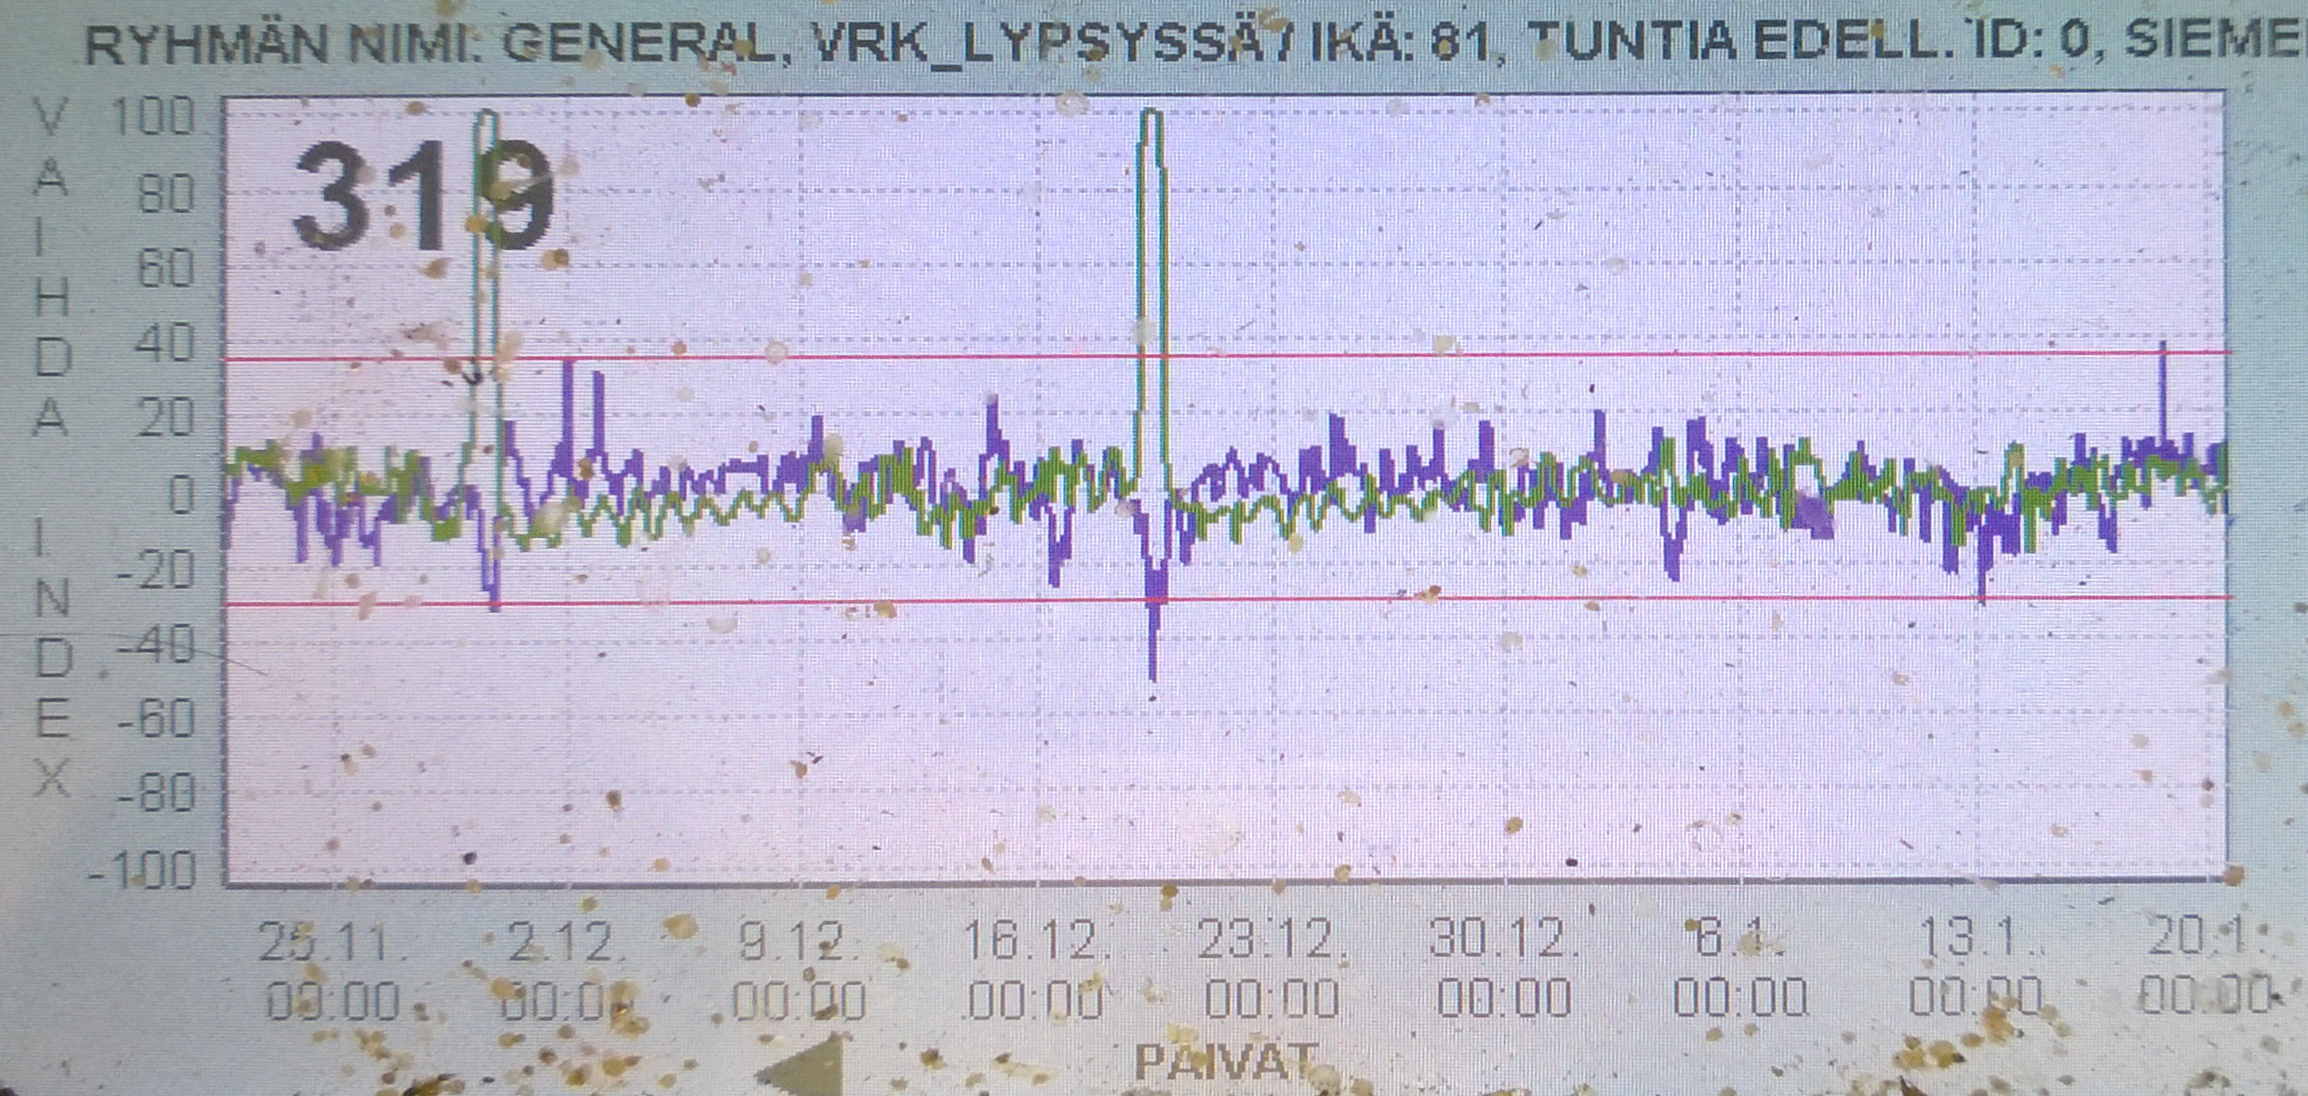
\includegraphics[width = 0.75\textwidth]{figures/heatime_kiima_319}
\caption{The activity data of Heatime system of the cow 319. The cow has had estruses approximately on October the 30\textsuperscript{th} and December the 20\textsuperscript{th}. The latter of the estruses should be detectable in this study, hence it is within our data recording period.}
\label{heatime_kiima_319}
\end{figure}

\begin{figure}[htb]
\centering
\includegraphics[width = 0.75\textwidth]{figures/kiimadata_319.png}
\caption{The raw acceleration data of each axis of the cow 319. The time frame of this picture is restricted around the estrus.}
\label{kiimadata_319}
\end{figure}


\begin{table} \caption{Increased activity periods detected with Heatime cow monitoring system. Increased activity is considered as proestrus. These detections are used as a reference in this study.} \label{fullestrustable}
\centering
\begin{tabular}{| p{1.25cm} | p{2.25cm} | p{9 cm} |}
\hline
\textbf{Cow ID} & \textbf{Occurrence of increased activity} & \textbf{Notifications} \\  \hline
319 & 30-11-2016 & High activity period considered as proestrus. However, this period is outside our sampling period. \\ \hline
319 & 19-12-2016 &  Second period of high activity considered as proestrus. This activity period is within our data recording period.  \\ \hline
9885 & 24-11-2016 & First high activity period of this cow and it is considered as a proestrus. However, the occurrence is outside our data recording period.  \\ \hline
9885  & 22-12-2016  & The second activity period of this cow is considered as proestrus. However, this activity period is delayed possibly because of stress cause by the new sensor. Nevertheless, the proestrus is within our data recording period.  \\ \hline
9885  & 04-01-2017  & Third high activity period of the cow 9885. In contrast to the previous occurrence, this is slightly early. However, also this occurrence is within our data recording period.  \\ \hline
 767 &  21-01-2017 & The first high activity period of this cow. Unfortunately, the occurrence is outside our data recording period.  \\ \hline
 767 & 13-02-2017  & The second activity period of this cow is within our data recording period.  \\ \hline
 787 & 08-01-2017 &  The first activity period of this cow. However, the amplitude of the activity is not very high. Therefore, it is considered as proestrus with restrictions. Additionally, the occurrence is outside our data recording period. \\ \hline
 787 & 19-01-2017  & The second increased activity period of the cow. This time the activity is high enough and the event should be considered as proestrus. However, also this occurrence is outside our data recording period.  \\ \hline
 787 & 10-02-2017  &  The third occurrence of increased activity of this cow. The occurrence is within our data recording period. Thus, it can be used as a reference in algorithm development. \\ \hline
\end{tabular}
\end{table}

Previously, we discussed of the activity periods detected by the Heatime system. However, it is only the reference for our own estrus detection algorithms. Therefore, the following subsections will evaluate the algorithms separately. However, in order to validate the results of the algorithms, it is mandatory to define the necessary measures of quality. Considering the estrus, the cow either is in proestrus or is not in proestrus. Thus, four simple but exact fundamental measures, \textit{true positive}, \textit{true negative}, \textit{false positive} and \textit{false negative} are suitable this evaluation. Furthermore, the definitions of the fundamental measurements are as follows.

\begin{itemize}
\item \textit{True positive} means a condition when the algorithm detects an ongoing estrus and the cow is in estrus.
\item \textit{True Negative} is a condition when the estrus detection algorithm yields negative for estrus and the cow is not in estrus.
\item \textit{False positive} states that the estrus detection algorithm yields positive for estrus but the cow is not in estrus.
\item \textit{False negative} means a condition when the estrus detection algorithm yields not in estrus but the cow is in estrus.
\end{itemize}
In addition to these fundamental measures, it is beneficial to have some additional descriptive evaluations for the algorithms. Thus, amplitude difference between normal and increased activity periods can describe the risk of false detections. 


The following subsections discusses of each estrus detection algorithm separately. The discussion includes the description of the performance and reliability of the algorithm. Additionally, we argue over the algorithm specific parameter configurations and their effect on the results. In this study the parameters are tuned with iterative methods. That is, testing various values and evaluating the results before applying new values. This iteration is continued until, the results are satisfactory and further tuning does not improve the results. Similarly, we attempt to reach some boundary vales for the parameters that increase the possibility of false results. The evaluation starts with the activity measurement algorithm. The algorithm rather straight forward and does not require advantageous computation. Next, we  evaluate the variance detection algorithm. The algorithm is based on the variance of periodic and short data samples. Thus, it is more complex than the first algorithm. Furthermore, it consists more tunable parameters than the first one. Lastly, we evaluate the inactivity detection algorithm. Despite the name of the algorithm, it attempts to detect lack of in activity, which corresponds the highly active proestrus period. Similarly, to the variance detection algorithm, the inactivity detection algorithm contains more tunable parameters than the first one. These parameters are discussed in the evaluation.


\subsubsection{Activity Monitoring} \label{activitymeasurementevaluation}

In this section, we evaluate the activity measurement based estrus detection algorithm. As discussed earlier, total of four cows were used in algorithm development, hence data of two cows were corrupted.  Luckily, the data of four cows consisted of five periods of increased activity that could be considered as proestrus. Thus, we have five detectable estruses. This algorithm is very straight forwarding and does not consist any complex phases except the high-pass filtering as an offset compensation. However, the high-pass filter consists of simple multiplications and summing the results. Thus, it is not that complex machine-wise. Furthermore, in real application the filtering is executed in the accelerometer with simple configurations. Therefore, the filtering should not be considered as s formal part of the algorithm. Nevertheless, the offset compensation is a necessary step, hence the offset would distort the results as discussed in the section \ref{activitymeasurementsection}.

In general, the activity monitoring algorithm performed the estrus detection satisfactorily. That is, it did not yield any false positive or false negative results according the logs of the Heatime system. An example of a detected estrus is represented in figure \ref{ActivityMonitoringCow787}. In this figure, the highly active proestrus period appears as a peak in the middle of the monitoring period. Additionally, the amplitude difference between the peak value and other periods are significant. Thus, in this case the risk of false positives and false negatives is minor. Furthermore, the timing of the detection correlates with the Heatime. However, the results were not this clear with all the cows. In the worst case the normal activity reached nearly the value of 0.6 whereas the maximum is 1. Thus, in that case there is obvious risk of false detection. 

\begin{figure}[htb]
\centering
\includegraphics[width = 0.75 \textwidth]{figures/ActivityMonitoringCow787.png}
\caption{The results of activity measurement of the cow 787. The difference between the estrus and rest of the period is most distinct within this algorithm. Thus, the risk of false positive and false negative results is least significant.}
\label{ActivityMonitoringCow787}
\end{figure}

Because this algorithm was highly straight forward it lacked real tunability of its parameters. However, the size of the sliding integration window was variable \ref{activitymeasurementsection}. Thus, the effect of different sizes of the integration window was tested with this algorithm. The results of different sized integration windows are represented in figure \ref{integrationwindows}. As seen in the figure, a long integration time delays the detection of the end of proestrus period and, consequently, delays the detection of the estrus. In this case, the \SI{36}{\hour} window delays the estrus detection past the actual estrus. Thus, the integration time is too long. Conversely, a short integration time yields the risk of triggering estrus too early. In this figure, there is a hollow section during the activity period. There is an obvious risk for this intermediate decremented to trigger the end of proestrus too soon. In conclusion, integration window from \SI{9}{\hour} to \SI{12}{\hour} is an optimal integration window. This conclusion correlates with the duration of the typical dairy cow proestrus.


\begin{figure}[htb]
\centering
\includegraphics[width = 0.75\textwidth]{figures/redcowactivity2.png}
\caption{The activity plots of the second proestrus of the cow 9885. The figure illustrates the effect of varying the size of the integration window. Wider window increases the amplitude of the estrus and eases the detectability. However, simultaneously it delays the moment of detection. }
\label{integrationwindows}
\end{figure}




\subsubsection{Variance Detection} \label{variancedetectionevaluation}

Above, we evaluated the results of the activity monitoring algorithm. The algorithm, is the simplest algorithm in this study and it is based on continuous data sampling. In general, the algorithm performed the estrus detection satisfactorily. However, it utilizes the micro-controller most of the time and therefore, it is not the preferred solution considering the power consumption. Conversely, the variance detection algorithm attempts to minimize the utilization of the micro-controller by using short and seldom data samples instead of continuous data streams. Consequently, this algorithm contains two more configurable variables than the activity monitoring algorithm.

The first configurable parameter is the size of the sample. The size of the sample has a major effect on the workload of the micro-controller. That is, the variance requires of calculating the mean value and as many square roots as the sample size. Furthermore, it requires working memory to store all the intermediate values prior yielding the final output value. Thus, the size of the sample shall remain as small as possible. However, it is possible that too small sample does not include enough of variation. Consequently, it might degrade the results. The second configurable parameter is the sampling interval. As already discussed, it is also possible to overlap the samples \ref{variancedetectionsection}. However, such an approach is against the attempt to reduce the utilization of the micro-controller. Otherwise, frequent sampling ensures all the behavior of the cow has being sampled and processed according the specifications of the algorithm. Nevertheless, seldom sampling improves the power saving capabilities of the micro-controller. However, the activities of the cow are likely missed with too seldom sampling hence, the cow moves infrequently and the moving time is relatively short. In conclusion, the purpose of tuning of the algorithm is to find the balance between sample size and sampling interval. An example of detected estrus with balanced variables in represented in figure \ref{VarianceDetectionCow767}. With the optimal values the algorithm did not yield any false results according the Heatime system. The sample size of 32 data points corresponds of two second sampling period whereas the sampling interval of 72 seconds is more than one minute. Consequently, the algorithm has reduced the amount of required samples by \SI{97.2}{\percent} in comparison to the activity monitoring algorithm.


\begin{figure}[htb]
\centering
\includegraphics[width = 0.75 \textwidth]{figures/VarianceDetectionCow767.png}
\caption{The variance detection results of the cow 767. There are multiple false positive detections in the data period. In general, there is no obvious difference between the estrus and non-estrus periods. Nevertheless, a true positive estrus is detected on February the 13\textsuperscript{th}.}
\label{VarianceDetectionCow767}
\end{figure}

In addition to searching the optimal values for the estrus detection, one objective is finding the boundary values for the algorithm. The boundary values are such that the algorithm becomes unstable and yields false results if the parameters are not within the boundaries. Figure \ref{VarianceDetectionCow767_32frames144seconds} represents one of the boundary solutions. That is, the algorithm has triggered a false estrus on February the 18\textsuperscript{th} because of too seldom sampling interval. However, increasing the sample size to 64 data points stabilizes the algorithm but is is more demanding for the micro-controller to calculate. Correspondingly, a sample of less than 16 data points yields false results with sampling interval of 32 seconds. However, decreasing the sampling interval to 24 seconds stabilized the algorithm. However, the sampling interval is three times more frequent in comparison to the optimal values.


\begin{figure}[htb]
\centering
\includegraphics[width = 0.75 \textwidth]{figures/VarianceDetectionCow767_32frames144seconds.png}
\caption{More seldom sampling yield false positive results as seen in this picture.}
\label{VarianceDetectionCow767_32frames144seconds}
\end{figure}

In general, the variance detection algorithm performed the estrus detection satisfactorily. However, in comparison to the activity monitoring algorithm, this algorithm showed marks of instability. Thus, the sample size and sampling interval shall be configured with care. Nevertheless, the algorithm capable of reducing the up-time of the micro-controller significantly. Therefore, it might be rather preferred option than the activity monitoring. Additionally, the amplitude difference between the peak value and the other periods remained within same values as it was with the fist algorithm. That is, the maximum value of non-proestrus period with the optimized parameters were 0.5 whereas it was 0.6 with the first algorithm.



%-----------------------------------------------------------------------%
\subsubsection{Inactivity Detection}\label{inactivitydetectionevaluation}

In contrast to the two previous algorithms, the inactivity detection has an alternative approach to the estrus detection. The first two algorithms are measuring the level of activity whereas this algorithm detects absence of activity. However, eventually the estrus detection is based in absence of inactivity. Finally, in could be considered as activity detection. Nevertheless, the other difference between inactivity detection and the other two algorithms is execution of the core functions of the algorithm in the accelerometer instead of utilizing the micro-controller. Therefore, the power saving capabilities if this algorithm is the highest in this study. Furthermore, the minimum interval between generated interrupts are configurable as discussed in section \ref{inactivitydetectionsection}. In result, the micro-controller books seldom interrupts and integrates them within the integration window of \SI{9}{\hour} to \SI{12}{\hour}. Additionally, the absence of interrupts is related to highly active proestrus behavior. Furthermore, in contrast to the first two algorithms, the peak value points downwards as seen in the figure \ref{InactivityDetectionCow9885}. The inactivity detection algorithm contains two configurable parameters, motion threshold and delay. In this figure the motion threshold is set to \SI{2}{\gram} and the delay is the maximum of \SI{336}{s}. As seen in the figure, the amplitude of non-proestrus periods is low in comparison to the two previous algorithms.


\begin{figure}[htb]
\centering
\includegraphics[width = 0.75 \textwidth]{figures/InactivityDetectionCow9885.png}
\caption{The results of inactivity detection algorithm of the cow 9885. The parameters are 336 second delay and \SI{2}{\gram} motion threshold. Both the estruses are detected as true positive on December the 22\textsuperscript{nd} and January the 4\textsuperscript{th}. No false positive or false negative detection occurred. The amplitude difference between proestrus and non-estrus is obvious.}
\label{InactivityDetectionCow9885}
\end{figure}

Furthermore, the inactivity detection algorithm seemed the most stable and reliable algorithm in this study. It was highly tolerable to the parameter configurations. Therefore, it did not yield any false results and it detected all true positive and true negative states. Eventually, only most irrational parameters yielded unstable behavior of the algorithm as seen in the figure \ref{InactivityDetectionCow9885_336period05threshold}. In this case, the motion threshold is as low as any motion of the cow. Thus, the no-motion conditions are not met that often. Similarly, if the motion threshold exceeds the normal motion values of the cow, \SI{4}{\gram}, the no-motion interrupts are always generated and therefore, there are no difference between proestrus and other periods. Additionally, decreasing of the delay had no significant impact on the results. Decreasing the delay only generates more interrupts and consequently, increases the up-time of the micro-controller and degrades the power saving capabilities. 

\begin{figure}[htb]
\centering
\includegraphics[width = 0.75 \textwidth]{figures/InactivityDetectionCow9885_336period05threshold.png}
\caption{}
\label{InactivityDetectionCow9885_336period05threshold}
\end{figure}

In summary, the inactivity detection algorithm is highly stable against parameter configurations. Furthermore, it was able to detect all the estruses. Moreover, the amplitude difference between proestrus and other periods were the most significant with this algorithm. The maximum non-proestrus amplitude with the optimized parameters was 0.2 whereas with other algorithms the amplitude was 0.6 and 0.5. Furthermore, this algorithm provides the highest capability for power saving. Firstly, the delay configuration defines the minimum interval between the interrupts, which is \SI{336}{\second}. That is, a maximum of 10.7 interrupts per hour. Secondly, the micro-controller is not required to perform any demanding calculations. It is only responsible of integrating the number of interrupt within the integration window of \SI{9}{\hour} to \SI{12}{\hour}. Thus, within all the measures of the quality an performance, the inactivity detection is the preferred algorithm for dairy cow estrus detection.


%-----------------------------------------------------------------------%
\section{Conclusions} \label{conclusionssection}

Previously, we discussed of the results of this study. The results included general and intermediate results that were used in algorithm development as well as in improvement of the sensor device software. Additionally, we evaluated the results of the estrus detection algorithms. This section summarizes the achieved results and draws comprehensive conclusions. First, we will discuss of sensor based estrus detection. The discussion will first evaluate the consent of sensor based estrus detection. Additionally, we will focus on the deficiencies of this study and propose corrective actions. Next, we will cover the occurred failures of this study. Moreover, we will discuss of some consideration related to data recording and wearable sensors in general. Lastly, in this section we propose suggestions for following studies.

%-----------------------------------------------------------------------%
\subsection{Sensor Based Estrus Detection}

This study introduced a sensor device for dairy cow estrus detection. The introduction included as well as the hardware configuration as well as the software implementation. Furthermore, we discussed of three different estrus detection algorithms suitable for the device. Practically, the algorithms were developed and tested with Matlab software on computer after recording of real cow data. The algorithms were different in their approach to the topic. However, all of them were based on the accelerometer data only. In summary, all the algorithms performed the estrus detection satisfactorily after tuning of the algorithm specific parameters. Nevertheless, there were some differences in the reliability as well as in the clearance of the results. Furthermore, the most significant differences between the algorithms were in the power saving capabilities, which is essential with battery-powered devices.

The activity monitoring based estrus detection algorithm was a straightforward integration of the accelerometer data. The only configurable parameter of the algorithm was the length of the integration time. In result, the most suitable integration time corresponds approximately the duration of the proestrus phase of the estrus cycle, that is roughly from 9 to \SI{12}{\hour}. Extending of the integration time only delayed the detection of estrus. Thus, it was not advisable option to follow. Conversely, integration time less than \SI{6}{\hour} yielded a risk of triggering estrus too early in the middle of the proestrus. These results of integration time were so obvious, that it was not tested with other algorithms. Moreover, it was decided to use \SI{9}{\hour} window with the rest of the algorithms. Furthermore, the algorithm was quite robust. That is, the results were mostly clear and there was no extremely high risk of yielding false results. However, the algorithm is sensitive to data offset and it shall be removed before any other computation. Fortunately, the accelerometer is capable of offset compensating. Thus, there is no need to implement it to the algorithm if it is considered in the configurations of the accelerometer.

In contrast to the activity monitoring algorithm, the variance detection algorithm was more complex. In contained two more configurable parameters. Furthermore, it was sensitive to the parameter configurations. Therefore, too small sample of too seldom sampling interval caused instability in the performance and increased the risk of false detections significantly. However, instability caused by seldom sampling interval was  possible to compensate in some matter with larger data samples. Accordingly, instability caused by short samples was possible to compensate with more frequent sampling interval. Nevertheless, the optimized parameters provided slightly better results in estrus detection. Furthermore, it provided significantly improved power saving capabilities for the micro-controller. Thus, the variance detection is more preferred estrus detection algorithm than the activity monitoring. However, the stability of the algorithm might require further testing with more cows.

Similarly, to the variance detection, the inactivity detection algorithm had two additional tunable parameters. However, inactivity detection seemed to be highly stable against the parameter configuration. In this study, any reasonable parameter values yielded true positive and true negative results with good clearance. Furthermore, no false results occurred with the reasonable parameter values. However, the most irrational parameter configurations were able to generate instability and decrease the clearance between proestrus and other activities. In conclusion, the performance and reliability of this algorithm was the most promising in this study. Furthermore, this algorithm is the most suitable for the micro-controller based solutions. That is, it requires a minimal amount of calculation of the micro-controller. In contrast, the core function of the algorithm is performed in the accelerometer. Thus, it enables the efficient use of power saving modes of the micro-controller which is critical with battery powered solutions. 

In summary, the estrus of a dairy cow is detectable with triaxial accelerometer. Furthermore, the estrus detection does not require confirmation of other sensors. However, the results were compared the  activity measurements of a single commercial system. Thus, the results cannot be declared as completely reliable and valid. Therefore, in order to receive valid results a veterinarian should confirmed all the detected estruses. That is, normally the cows are inseminated after estrus detection. In result of successful insemination, the following pregnancy confirms timely estrus detection. Additionally, the estrus detection algorithms developed in this study are highly suitable for micro-controller based devices. The complexion and the requirement of computation power were considered already in the development phase. Furthermore, the complexity did not correlate with the performance of the algorithm. The lightest algorithm was also the most reliable and effective. Moreover, the estrus detection device does not require large data storage such as SD-card to store the data. The internal memory is sufficient with these applications.

%-----------------------------------------------------------------------%
\subsection{Failures and considerations}

Previously, we draw conclusions of sensor based dairy cow estrus detection. In general, all the algorithms developed in this study were successful in the estrus detection. By contrast to the success in estrus detection, this subsection discusses of the failures and deficiencies of this study. First, we will discuss of the temperature measurements as the verification for the estrus detection. Next, we attempt to infer the reason for several corrupted sets of data during the data recording events. Lastly, we will consider some imperfections of the device hardware design. 

In general, the skin temperature measurements were a total failure in this study. That is, the heat conducting tape did not conduct the heat enough. Conversely, the results of the temperature measurements seemed to follow something else instead. Similar temperature curve was also seen in the measurements of the accelerometer \ref{temperaturemeasurements}. Hence the bot measurements were synchronous, it was concluded the measurements most likely followed the air temperature of the cowshed rather than the skin temperature of the cow. Additionally, it was tested to filter the results and calculate the differential of the two temperatures sensors. Nevertheless, no correlation was found between the temperature measurements and the ongoing estrus or proestrus in this study. Replacing the temperature sensor directly against the skin of the cow could improve the results. However, ensuring a proper continuous skin contact is till questionable. Nevertheless, the differential of the measurements of temperature sensor and accelerometer would more likely provide a possibility to estimate the skin temperature with adequate estimation algorithm. However, complex estimators may not be suitable for micro-controller based solutions. Thus, the temperature sensor is a redundant component and could be removed from the hardware design.

In this study, a total of three cow data records were partially corrupted and the data was not valid in algorithm development. Unfortunately, there were no proper methods to directly define the cause of the error. However, further investigation implied that the device software continued its normal exaction all the time. By contrast, it seemed that the accelerometer had somehow reset its configurations. However, this conclusion is not obvious, hence the main reason for unexpected resetting would be a power failure. Furthermore, normal power failure would reset all the components of the device. Consequently, the micro-controller would have re-configured the accelerometer and the device would have been working normally. Therefore, it is difficult to explain why the accelerometer would have reset but micro-controller not. Nevertheless, in result, the micro-controller stopped receiving interrupt from the accelerometer. Consequently, the micro-controller software met the time-out condition, which forced the micro-controller to read the FIFO buffer of the accelerometer. However, because of resetting, the FIFO buffer contained only single data frame. Thus, the log file consists of one frame of acceleration measurements in sequence of temperature measurements. If we consider the interval between the timeout condition the time span of the corrupted log corresponds the duration of the data recording event. Thus, this explanation is highly possible reason. In future, the device software should enhance with a function that is capable to detect false sensor configurations and re-configure the sensor whenever necessary.


Furthermore, the hardware design did not provide optimal performance for high sampling rate as seen in the results \ref{generalresultssection}. The duration of SD file operations exceeded the filling time of the FIFO buffer off the accelerometer. Thus, the first recorded set of data was partially corrupted because of frequent buffer overflows. Additionally, a high sampling rate fulfilled the SD memory card relatively fast and increasing the size of the SD card would not necessary be the optimal solution. Thus, if a high sampling rate is needed, there is a need to look for other solutions than SD-memory card.


%-----------------------------------------------------------------------%
\subsection{Suggestions for Future Studies}


As discussed earlier, the estruses detection in this study was never properly confirmed. Conversely, the results were verified only with another sensor device which acted as a reference in this study. Therefore, the results of this study are not completely reliable. One option for following studies would be the verification of the developed algorithms. In order to validate the algorithms, they should be implemented directly on micro-controller. Furthermore, the algorithms should be tested in real-time with real dairy cattle instead of posterior data processing on computer. Furthermore, the validation would require controlling of the detections. It means that the cow with detected estrus should be inseminated and a successful pregnancy is finally the only proper validation of estrus detection. Usually, early confirmation of pregnancy would require examination of a veterinarian. Nevertheless, still we would need to consider the normal success rate of insemination.

Furthermore, the amount of data used for algorithm development was quite small. That is, only four months of cow data was valid to use in algorithm development. Luckily, the data consisted total of five estruses. Nevertheless, statistically the amount of data is rather minor considering the headcount worldwide. Therefore, it is likely that there is even more variance in the cow activity levels than it was in this study. Additionally, we should consider other breeds as well. furthermore, the cows in this study had no free access to the pasture. Thus, the results might differ with the cows on pasture. Thus, another option for following studies is recording more of cow data considering various breeds and environments. Furthermore, our study normalized all the results. Thus, the actual difference of activity levels between the cows were not considered in this study. Therefore, the algorithms are not directly convertible to the micro-controller, hence, we do not know proper thresholds. Furthermore, one significant improvement would be using adjustable thresholds instead of fixed ones. The real-time adjustability would require applying of filter or estimator of the cow's behavior.

Lastly, the behavior monitoring was considered as a secondary objective in this study. However, the behavior monitoring failed in lack of proper time synchronization. Nevertheless, there seemed to be correlation between certain behaviors and the characteristics in the data. Thus, the third suggestion for following studies is developing behavior monitoring algorithms. In order to achieve proper time synchronization, the sensor device should be enhanced with backup powered real-time clock. Additionally, the video recording device should contain similar real-time clock and the initial time should be synchronized prior recording the data. Furthermore, the collar of the cow may not be the optimal mounting point for the camera. Same applies with the ceiling camera in large cowshed. Nevertheless, the resolution is somewhere between these two options. However, the continuous tracking of the animal is one of the essential criteria.


\clearpage

%-----------------------------------------------------------------------%
%\section{Summary} \label{summarysection}


%Summary of all the previous. Alternatively ``Discussion'' or ``Conclusions''...


\clearpage
%% Lähdeluettelo

\thesisbibliography
\printbibliography




%% Liitteet
\clearpage

\thesisappendix

%%
%\section{Esimerkki liitteestä\label{LiiteA}}
%
%Liitteet eivät ole opinnäytteen kannalta välttämättömiä ja 
%opinnäytteen tekijän on 
%kirjoittamaan ryhtyessään hyvä ajatella pärjäävänsä ilman liitteitä.
%Kokemattomat kirjoittajat, jotka ovat huolissaan
%tekstiosan pituudesta, paisuttavat turhan 
%helposti liitteitä pitääkseen tekstiosan pituuden annetuissa rajoissa.
%Tällä tavalla ei synny hyvää opinnäytettä.   
%
%Liite on itsenäinen kokonaisuus, vaikka se täydentääkin tekstiosaa.
%Liite ei siten ole pelkkä listaus, kuva tai taulukko, vaan 
%liitteessä selitetään aina sisällön laatu ja tarkoitus. 
%
%Liitteeseen voi laittaa esimerkiksi listauksia. Alla on 
%listausesimerkki tämän liitteen luomisesta. 
%
%%% Verbatim-ympäristö ei muotoile tai tavuta tekstiä. Fontti on monospace.
%%% Verbatim-ympäristön sisällä annettuja komentoja ei LaTeX käsittele. 
%%% Vasta \end{verbatim}-komennon jälkeen jatketaan käsittelyä.
%\begin{verbatim}
%	\clearpage
%	\appendix
%	\addcontentsline{toc}{section}{Liite A}
%	\section*{Liite A}
%	...
%	\thispagestyle{empty}
%	...
%	tekstiä
%	...
%	\clearpage
%\end{verbatim}
%
%Kaavojen numerointi muodostaa liitteissä oman kokonaisuutensa:
%\begin{eqnarray}
%d \wedge A  &=& F, \label{liitekaava1}\\
%d \wedge F  &=& 0. \label{liitekaava2}
%\end{eqnarray}
%
%
%\clearpage
%\section{Toinen esimerkki liitteestä\label{LiiteB}}
%
%%% Liitteiden kaavat, taulukot ja kuvat numeroidaan omana kokonaisuutenaan
%
%Liitteissä voi myös olla kuvia, jotka
%eivät sovi leipätekstin joukkoon:
%%% Ympäristön figure parametrit htb pakottavat
%%% kuvan tähän, eikä LaTeX yritä siirrellä niitä
%%% hyväksi katsomaansa paikkaan. 
%%% Ympäristöä center voi käyttää \centering-
%%% komennon sijaan
%%%
%\begin{figure}[htb]
%\begin{center}
%\includegraphics[height=8cm]{kuva2}
%\end{center}
%\caption{Kuvateksti, jossa on liitteen numerointi}
%\label{liitekuva}
%\end{figure}
%%%
%Liitteiden taulukoiden numerointi on kuvien ja kaavojen kaltainen:
%\begin{table}[htb]
%\caption{Taulukon kuvateksti.}
%\label{liitetaulukko}
%\begin{center}
%\fbox{
%\begin{tabular}{lp{0.5\linewidth}}
%9.00--9.55  & Käytettävyystestauksen tiedotustilaisuus (osanottajat
%ovat saaneet sähköpostitse valmistautumistehtävät, joten tiedotustilaisuus
%voidaan pitää lyhyenä).\\
%9.55--10.00 & Testausalueelle siirtyminen
%\end{tabular}}
%\end{center}
%\end{table}
%Kaavojen numerointi muodostaa liitteissä oman kokonaisuutensa:
%\begin{eqnarray}
%T_{ik} &=& -p g_{ik} + w u_i u_k + \tau_{ik},  \label{liitekaava3} \\
%n_i    &=& n u_i + v_i.                      \label{liitekaava4}
%\end{eqnarray}


\end{document}
